\documentclass[
	% -- opções da classe memoir --
	12pt,					% tamanho da fonte
	openright,				% capítulos começam em pág ímpar (insere página vazia caso preciso)
	oneside,					% para impressão em verso e anverso. Oposto a oneside
	a4paper,					% tamanho do papel. 
	% -- opções da classe abntex2 --
	%chapter=TITLE,			% títulos de capítulos convertidos em letras maiúsculas
	%section=TITLE,			% títulos de seções convertidos em letras maiúsculas
	%subsection=TITLE,		% títulos de subseções convertidos em letras maiúsculas
	%subsubsection=TITLE,	% títulos de subsubseções convertidos em letras maiúsculas
	% -- opções do pacote babel --
	english,					% idioma adicional para hifenização
	%french,					% idioma adicional para hifenização
	%spanish,				% idioma adicional para hifenização
	brazil					% o último idioma é o principal do documento
	]{abntex2}

% ---------------------
% Pacotes OBRIGATÓRIOS
% ---------------------
\usepackage{lmodern}			% Usa a fonte Latin Modern			
\usepackage[T1]{fontenc}		% Selecao de codigos de fonte.
\usepackage[utf8]{inputenc}		% Codificacao do documento (conversão automática dos acentos)
\usepackage{lastpage}			% Usado pela Ficha catalográfica
\usepackage{indentfirst}		% Indenta o primeiro parágrafo de cada seção.
\usepackage{color}				% Controle das cores
\usepackage{graphicx,graphicx}	% Inclusão de gráficos
\usepackage{epsfig,subfig}		% Inclusão de figuras
\usepackage{microtype} 			% Melhorias de justificação
\usepackage{verbatim}           % Comentarios de mais de uma linha
% ---------------------
		
% ---------------------
% Pacotes ADICIONAIS
% ---------------------
\usepackage{listings}                   % https://www.overleaf.com/learn/latex/Code_listing
\usepackage{lipsum}						% Geração de dummy text
\usepackage{amsmath,amssymb,mathrsfs}	% Comandos matemáticos avançados 
\usepackage{setspace}  					% Para permitir espaçamento simples, 1 1/2 e duplo
\usepackage{tabularx} 					% Para poder ter tabelas com colunas de largura auto-ajustável
\usepackage{multirow}                   % 
\usepackage{afterpage} 					% Para executar um comando depois do fim da página corrente
\usepackage{url} 						% Para formatar URLs (endereços da Web)
\usepackage[table]{xcolor}
\usepackage{float}                      % Para colocar imagens exatamente na posição desejada
\usepackage{mathtools}                  % Símbolos matemáticos
\usepackage{colortbl}                   % Colorir células de tabelas
\usepackage{color}
\usepackage{array}
% ---------------------


% ---------------------
% Pacotes de CITAÇÕES
% ---------------------
\usepackage[brazilian,hyperpageref]{backref}	% Paginas com as citações na bibl
\usepackage[alf]{abntex2cite}					% Citações padrão ABNT (alfa)
%\usepackage[num]{abntex2cite}					% Citações padrão ABNT (numericas)
% ---------------------

% Configurações de CITAÇÕES para abntex2
% --- 
% CONFIGURAÇÕES DE PACOTES
% --- 

% ---
% Configurações do pacote backref
% Usado sem a opção hyperpageref de backref
\renewcommand{\backrefpagesname}{Citado na(s) página(s):~}
% Texto padrão antes do número das páginas
\renewcommand{\backref}{}
% Define os textos da citação
\renewcommand*{\backrefalt}[4]{
	\ifcase #1 %
		Nenhuma citação no texto.%
	\or
		Citado na página #2.%
	\else
		Citado #1 vezes nas páginas #2.%
	\fi}%
% ---

% Inclusão de dados para CAPA e FOLHA DE ROSTO (título, autor, orientador, etc.)
% ---
% Informações de dados para CAPA e FOLHA DE ROSTO
% ---
\titulo{Análise de Sentimentos Temporal a partir de Avaliações Online de Hotéis no Google Maps}
\autor{Emerson Almeida Matos}
\local{Santo André - SP}
\data{Novembro de 2024} % TODO
\orientador{Alexandre Donizeti Alves}
%\coorientador{Fulano Nome do Coorientador}
\instituicao{%
  Universidade Federal do ABC -- UFABC
  \par
  Centro de Matemática, Computação \& Cognição 
  \par
  Bacharelado em Ciência da Computação}
\tipotrabalho{Projeto de Graduação em Computação}
% O preambulo deve conter o tipo do trabalho, o objetivo,
% o nome da instituição e a área de concentração
\preambulo{\textbf{Projeto de Graduação em Computação} apresentado como parte dos requisitos necessários para a obtenção do Título de Bacharel em Ciência da Computação.}
% ---


% Inclui Configurações de aparência do PDF Final
%  Configurações de aparência do PDF final
% NÃO ALTERAR!!!

% alterando o aspecto da cor azul
\definecolor{blue}{RGB}{41,5,195}

% informações do PDF
\makeatletter
\hypersetup{
     	%pagebackref=true,
		pdftitle={\@title}, 
		pdfauthor={\@author},
    		pdfsubject={\imprimirpreambulo},
	    pdfcreator={LaTeX with abnTeX2},
		pdfkeywords={abnt}{latex}{abntex}{abntex2}{trabalho acadêmico}, 
		colorlinks=true,       		% false: boxed links; true: colored links
    		linkcolor=blue,          	% color of internal links
    		citecolor=blue,        		% color of links to bibliography
    		filecolor=magenta,      		% color of file links
		urlcolor=blue,
		bookmarksdepth=4
} 
\makeatother
% --- 

% Inclui Configurações para o listing
% ---
% CONFIGURAÇÕES DE PACOTES
% ---

%New colors defined below
\definecolor{codegreen}{rgb}{0,0.6,0}
\definecolor{codegray}{rgb}{0.5,0.5,0.5}
\definecolor{codepurple}{rgb}{0.58,0,0.82}
\definecolor{backcolour}{rgb}{0.95,0.95,0.92}

%Code listing style named "mystyle"
\lstdefinestyle{mystyle}{
  backgroundcolor=\color{backcolour},
  commentstyle=\color{codegreen},
  keywordstyle=\color{magenta},
  numberstyle=\tiny\color{codegray},
  stringstyle=\color{codepurple},
  basicstyle=\ttfamily\footnotesize,
  breakatwhitespace=false,
  breaklines=true,
  captionpos=b,
  keepspaces=true,
  numbers=left,
  numbersep=5pt,
  showspaces=false,
  showstringspaces=false,
  showtabs=false,
  tabsize=2
}

\lstset{style=mystyle}


% O tamanho da identação do parágrafo é dado por:
\setlength{\parindent}{1.3cm}

% Controle do espaçamento entre um parágrafo e outro:
\setlength{\parskip}{0.2cm}  % tente também \onelineskip

% ---------------------
% Compila o indice
% ---------------------
\makeindex
% ---------------------

%%%%%%%%%%%%%%%%%%%%%%%%%%%
%%  INICIO DO DOCUMENTO  %%
%%%%%%%%%%%%%%%%%%%%%%%%%%%
\begin{document}

% Retira espaço extra obsoleto entre as frases.
\frenchspacing

% ----------------------------------------------------------
% ELEMENTOS PRÉ-TEXTUAIS (Capa, Resumo, Abstract, etc.)
% ----------------------------------------------------------
\pretextual

% Capa
% ---
% Impressão da Capa
% ---
  \begin{capa}%
    \begin{figure}[h!]%
        \centering%
        
\includegraphics[scale=1.2]{figs/logo.png}%
      \end{figure}%
    \center
	\ABNTEXchapterfont\large{Universidade Federal do ABC \\ Centro de Matemática, Computação \& Cognição \\ Bacharelado em Ciência da Computação}
	%\vspace{1.5cm}

    \vfill
    \ABNTEXchapterfont\bfseries\LARGE\imprimirtitulo
    \vfill

	%\vfill
	\ABNTEXchapterfont\large\imprimirautor
	\vfill
%
	
	
    \large\imprimirlocal, \large\imprimirdata

    \vspace*{1cm}
  \end{capa}
% ---

% Folha de rosto (o * indica que haverá a ficha bibliográfica)
\imprimirfolhaderosto*



% Imprimir Ficha Catalografica
% ---
% Ficha Catalográfica
% ---
% Isto é um exemplo de Ficha Catalográfica, ou ``Dados internacionais de
% catalogação-na-publicação''. Você pode utilizar este modelo como referência. 
% Porém, talvez a biblioteca lhe fornece um PDF
% com a ficha catalográfica definitiva após a defesa do trabalho. Quando estiver
% com o documento, salve-o como PDF no diretório do seu projeto e substitua todo
% o conteúdo de implementação deste arquivo pelo comando abaixo:
%
% \begin{fichacatalografica}
%     \includepdf{fig_ficha_catalografica.pdf}
% \end{fichacatalografica}
\begin{fichacatalografica}
	\vspace*{\fill}					% Posição vertical
	\hrule							% Linha horizontal
	\begin{center}					% Minipage Centralizado
	\begin{minipage}[c]{12.5cm}		% Largura
	
	\imprimirautor
	
	\hspace{0.5cm} \imprimirtitulo  / \imprimirautor. --
	\imprimirlocal, \imprimirdata-
	
	\hspace{0.5cm} \pageref{LastPage} p. : il. (algumas color.) ; 30 cm.\\
	
	\hspace{0.5cm} \imprimirorientadorRotulo~\imprimirorientador\\
	
	\hspace{0.5cm}
	\parbox[t]{\textwidth}{\imprimirtipotrabalho~--~\imprimirinstituicao,
	\imprimirdata.}\\
	
	\hspace{0.5cm}
		1. Análise de sentimento.
            2. Processamento de Linguagem Natural
		3. Grandes modelos de linguagem.
            4. Google Maps
		5. GPT.
		6. Vicuna.
		7. OpenChat.
		8. BERT.
		I. Alexandre Donizeti Alves.
		II. Universidade Federal do ABC.
		III. UFABC.
		IV. Título de Bacharel em Ciência da Computação\\
	
	\hspace{8.75cm} CDU 02:141:005.7\\
	
	\end{minipage}
	\end{center}
	\hrule
\end{fichacatalografica}
% ---

% Inserir Folha de Aprovação
% ---
% Assinaturas
% ---
% Isto é um exemplo de Folha de aprovação, elemento obrigatório da NBR
% 14724/2011 (seção 4.2.1.3). Você pode utilizar este modelo até a aprovação
% do trabalho. Após isso, substitua todo o conteúdo deste arquivo por uma
% imagem da página assinada pela banca com o comando abaixo:
%
% \includepdf{folhadeaprovacao_final.pdf}
%
\begin{folhadeaprovacao}

  \begin{center}
    {\ABNTEXchapterfont\large\imprimirautor}

    \vspace*{\fill}\vspace*{\fill}
    \begin{center}
      \ABNTEXchapterfont\bfseries\Large\imprimirtitulo
    \end{center}
    \vspace*{\fill}
    
    \hspace{.45\textwidth}
    \begin{minipage}{.5\textwidth}
        \imprimirpreambulo
    \end{minipage}%
    \vspace*{\fill}
   \end{center}
        
 % Isso na versao final do trabalho!!!       
   Trabalho aprovado. \imprimirlocal, 01 de Novembro de 2024::

   \assinatura{\textbf{\imprimirorientador} \\ Orientador} 

   \assinatura{\textbf{Professor} \\ Convidado 1}
   \assinatura{\textbf{Professor} \\ Convidado 2}
   
      
   \begin{center}
    \vspace*{0.5cm}
    {\large\imprimirlocal}
    \par
    {\large\imprimirdata}
    \vspace*{1cm}
  \end{center}
  
\end{folhadeaprovacao}
% ---

% Dedicatória
% ---
% Dedicatória
% ---
\begin{dedicatoria}
   \vspace*{\fill}
   \centering
   \noindent
   \textit{Dedico este trabalho de conclusão de curso à minha família, amigos e professores, cujo apoio, incentivo e orientação foram fundamentais para a realização deste projeto. A todos vocês, meu sincero agradecimento.} \vspace*{\fill}
\end{dedicatoria}
% ---


% Agradecimentos
% ---
% Agradecimentos
% ---
\begin{agradecimentos}



Agradeço a Xuxa, meus pais, cachorro, gato e papagaio, por ...

Agradeço ao meu orientador, XXXXXXXXX, por todos os conselhos, pela paciência e ajuda nesse período.

Aos meus amigos ...

Aos professores ...

À XXXXXX pelo apoio financeiro para realização deste trabalho de pesquisa.

\end{agradecimentos}
%% ---

% Epígrafe
% ---
% Epígrafe
% ---
\begin{epigrafe}
    \vspace*{\fill}
	\begin{flushright}
		\textit{``Não sei o que, \\
		          não sei o que,\\
                  não sei o que lá.''\\
		          (Autor Desconhecido)}
	\end{flushright}
\end{epigrafe}
% ---

% Resumo e Abstract
% ---
% RESUMOS
% ---

% RESUMO em português
\setlength{\absparsep}{18pt} % ajusta o espaçamento dos parágrafos do resumo
\begin{resumo}

Este projeto pretende desenvolver um processo de análise de sentimentos temporal aplicado às avaliações online de hotéis no \textit{Google Maps}. Com o crescente volume de dados disponíveis em plataformas de avaliação, como \textit{Google Maps}, há a necessidade de entender como as opiniões de usuários evoluem ao longo do tempo, auxiliando novos clientes a tomarem decisões mais informadas. Para tanto, o trabalho propõe a utilização de modelos de Processamento de Linguagem Natural (PLN), incluindo modelos baseados em \textit{BERT} e outros modelos de linguagem de última geração, como \textit{GPT-3.5},\textit{OpenChat} e \textit{Vicuna}, para realizar a classificação dos sentimentos expressos nas avaliações. Além disso, são analisadas as variações temporais das avaliações, possibilitando identificar tendências e mudanças no comportamento dos usuários ao longo do tempo. A metodologia inclui a coleta automatizada de dados do \textit{Google Maps}, pré-processamento das informações e a aplicação dos modelos PLN para a extração dos sentimentos. Os resultados evidenciam a predominância de avaliações positivas e revelam padrões temporais nas opiniões dos clientes. Conclui-se que a análise de sentimentos temporal oferece uma visão valiosa para empresas e usuários, proporcionando percepções sobre a qualidade do serviço ao longo do tempo.



 \textbf{Palavras-chaves}: Análise de sentimento, Processamento de Linguagem Natural, Grandes modelos de linguagem, Google Maps, GPT, Vicuna, OpenChat, BERT.
\end{resumo}

% ABSTRACT in english
\begin{resumo}[Abstract]
 \begin{otherlanguage*}{english}
    This project aims to develop a process for temporal sentiment analysis applied to online reviews of hotels available on Google Maps. With the increasing volume of data on review platforms like Google Maps, there is a need to understand how user opinions evolve over time, helping new customers make more informed decisions. Therefore, this work proposes the use of Natural Language Processing (NLP) models, including \textit{BERT-based} models and other state-of-the-art language models like GPT-3.5, OpenChat and Vicuna, to classify the sentiments expressed in the reviews. Additionally, the temporal variations in reviews are analyzed, allowing the identification of trends and shifts in user behavior over time. The methodology includes automated data collection from Google Maps, data pre-processing, and the application of NLP models to extract sentiments. The results show a predominance of positive reviews and reveal temporal patterns in customer opinions. It is concluded that temporal sentiment analysis provides valuable insights for companies and users, offering an understanding of service quality over time.

   \vspace{\onelineskip}
 
   \noindent 
   \textbf{Keywords}: Sentiment analysis, Natural Language Processing, Large language models, Google Maps, GPT, Vicuna, OpenChat, BERT.
 \end{otherlanguage*}
\end{resumo}

% Lista de ilustrações
\pdfbookmark[0]{\listfigurename}{lof}
\listoffigures*
\cleardoublepage

% Lista de tabelas
\pdfbookmark[0]{\listtablename}{lot}
\listoftables
\cleardoublepage

% Lista de abreviaturas e siglas
\begin{siglas}
	\item[API] Application Programming Interface (Interface de Programação de Aplicação)
	\item[BERT] Bidirectional Encoder Representations from Transformers
	\item[CETIC] Centro Regional de Estudos para o Desenvolvimento da Sociedade da Informação
	\item[COVID-19] Doença por coronavirus (Coronavirus disease 2019)
	\item[GPT] Generative Pre-trained Transformer
	\item[LLaMa] Large Language Model Meta AI
	\item[LLM] Large Language Models (Grandes Modelos de Linguagem)
	\item[LMSYS] Large Model Systems Organization
	\item[LSTM] Long short-term memory
	\item[NLP] Natural language processing
	\item[PLN] Processamento de linguagem natural
	\item[SVM] Support Vector Machine
	\item[VADER] Valence Aware Dictionary and sEntiment Reasoner
\end{siglas}

% Lista de símbolos
%\begin{simbolos}
%	\item[$ \Gamma $] Letra grega Gama
%	\item[$ \Lambda $] Lambda
%	\item[$ \zeta $] Letra grega minúscula zeta
%	\item[$ \in $] Pertence
%\end{simbolos}
\begin{comment}
\end{comment}

% Inserir o SUMÁRIO
\pdfbookmark[0]{\contentsname}{toc}
\tableofcontents*
\cleardoublepage

% ----------------------------------------------------------
% ELEMENTOS TEXTUAIS (Capítulos)
% ----------------------------------------------------------
\textual
% Elementos textuais com numeração arábica
\pagenumbering{arabic}
% Reinicia a contagem do número de páginas
\setcounter{page}{1}


% Inclui cada capitulo do Trabalho
% ----------------------------------------------------------
% Introdução 
% Capítulo sem numeração, mas presente no Sumário
% ----------------------------------------------------------

\chapter[Introdução]{Introdução}
\label{cap:intro}
% \addcontentsline{toc}{chapter}{Introdução}
% pesquisa https://agenciabrasil.ebc.com.br/geral/noticia/2020-05/brasil-tem-134-milhoes-de-usuarios-de-internet-aponta-pesquisa#:~:text=Os%20recursos%20mais%20utilizados%20s%C3%A3o,eletr%C3%B4nico%20(39%25)%20e%20participa%C3%A7%C3%A3o
% https://cetic.br/pt/tics/domicilios/2021/individuos/C6/
% https://books.google.com.br/books?hl=pt-BR&lr=&id=cHYqBF3G3lkC&oi=fnd&pg=PR7&dq=facilidade+no+acesso+a+informacao&ots=g9ggkZ8lS0&sig=-GlYLDNbFKs0q5WYfttQiXkphdI#v=onepage&q=facilidade%20no%20acesso%20a%20informacao&f=false

\begin{comment}
Neste capítulo precisamos:
\begin{itemize}
    \item Introduzir o contexto
    \item Definir o que entendemos como avaliação de hotéis
    \item Apresentar em linhas gerais quais métodos são usados para detectar fake news, qual o estado da arte atual e quais são suas limitações.
    \item Descrever a nossa proposta e objetivos
    \item Descrever a estrutura do relatório.
\end{itemize}

\end{comment}

Com os avanços da tecnologia, o acesso à informação tem sido cada vez mais facilitado entre a população geral. Antes, as fontes de informações mais frequentes eram o conhecimento de prévio de indivíduos mais experientes ou conteúdos impressos. Uma pesquisa feita pela CETIC \cite{cetic2019pesquisa} indicava que 3 entre cada 4 brasileiros possuem acesso à internet e esses entrevistados também responderam que realizaram algum tipo de consulta online, onde 28\% procurou por informações referentes a viagens e acomodações, um índice baixo se comparado aos 57\% que respondeu ter buscado por informações sobre produtos e serviços.

% https://blog.buscaonibus.com.br/melhores-sites-de-hospedagem-para-sua-viagem/

Quando surge o interesse em realizar viagens, sites como TripAdvisor, Trivago, Booking, AirBnb e Google Local Guides, são as principais fontes de informações para locais ainda desconhecidos. É feita uma busca de informações de pessoas que já frequentaram os locais, onde cada usuário da plataforma preenche as avaliações conforme o modelo disponível em cada plataforma, partindo de uma avaliação objetiva dividida por categorias, onde o usuário é questionado por área de interesse de modo a atribuir um valor número como nota para aquela experiência, em muitos casos, existindo um bloco de texto disponível para relatar a experiência em sua estadia local. As plataformas citadas costumam ter, além das avaliações dos usuários, informações próprias onde a plataforma preenche, incluindo informações de preços por diárias e distâncias de atrações.

Essas informações costumam direcionar o internauta e o auxiliam em sua tomada de decisão, porém qual a validade dessas informações? como essas avaliações variam durante o tempo? esse hotel está tendo avaliações melhores agora do que no mesmo período no ano passado? esse local está sendo avaliado negativamente por conta de algum evento atípico? mesmo registrando uma avaliação ruim, o usuário que a submeteu possui outra avaliação registrada no passado?

Contudo, as plataformas nem sempre expõem as informações claras e objetivas, dificultando a tomada de decisões para o internauta, que possui o objetivo de escolher um local que contemple suas necessidades durante seu período de viagem, afinal, o internauta não tem interesse em ser surpreendido que as avaliações dispostas estavam equivocadas e as informações mais recentes tenham sido ocultadas devido às tendências negativas por conta da organização por nível de popularidade nas plataformas.

\begin{comment}
O presente relatório está estruturado da seguinte forma: o capítulo~\ref{cap:justificativa} apresenta..., o capítulo~\ref{cap:fund_teorica} ... O capítulo~\ref{cap:metodologia} ..., o capítulo~\ref{cap:resultados} ... O capítulo~\ref{cap:conclusao} 

Demonstração de citação: o software de análise foi desenvolvido na linguagem Python~\cite{van1995python}, usando as bibliotecas Pandas~\cite{mckinney2010data} e Scikit-learn~\cite{scikit-learn}.
\end{comment}

\begin{comment}
    como o sentimento dos usuários que avaliaram o estabelecimento variou durante o tempo, se o recinto está recebendo avaliações com sentimentos mais positivos ou se a tendência é de que as avaliações continuem com sentimentos cada vez mais negativos, e identificar possíveis mudanças de comportamento, que para esses cenários podem ser justificados por mudanças de equipe, mudanças de políticas internas da empresa ou por uma simples manutenção ou evolução das instalações
    , a fim de observar e entender as variações de sentimentos das avaliações realizadas pelos usuários da plataforma distribuídos durante o tempo.
\end{comment}

\section{Justificativa}
\begin{comment}
Estamos vivendo em um mundo com muitas informações disponíveis e de fácil acesso, porém esta cada vez mais difícil filtrar e escolher as informações que vão fornecer mais insumo para o internauta.
\end{comment}


\section{Estrutura da Monografia}

123
%\include{capitulos/justificativa}
%\chapter{Cronograma}
\label{cap:cronograma}

% \begin{figure}[h]
    % \center
    % \includegraphics[width=17cm]{figs/cronograma.png}
% \end{figure}

Inicialmente, será criado um corpus para análise com conteúdo suficiente para obter variação significativa nos sentimentos com o avanço do tempo, para ser possível identificar visualmente essas variações por hotel, tópico e por região.

Após essa etapa será necessário realizar o tratamento dos dados e o treinamento do modelo BERT para realizar a classificação do corpus.

Com o treinamento concluído, espera-se realizar o emparelhamento de adjetivo-substantivo e a avaliação de sentimento deles e de todo o corpus.

Com os resultados em mãos, será realizada um agrupamento por região e hotéis, visando mostrar de forma gráfica como essas avaliações têm variado temporalmente.

De forma resumida, o seguinte cronograma de atividades deverá ser considerado:

\begin{table}[H]
    \centering
    {\footnotesize
    \begin{tabular}{|p{6.1cm}|l|l|l|l|l|l|l|l|l|l|l|l|}
    \hline
    \multirow{2}{*}{ATIVIDADES} & \multicolumn{5}{c|}{PGC II} & \multicolumn{4}{c|}{PGC III}\\ \cline{2-10}
                                           &Set&Out&Nov&Dez&Jan&Jun&Jul&Ago&Set \\ \hline
    1. Conjunto de Dados                   & X & X & X &   &   &   &   &   &    \\ \hline
    2. Pré-processamento dos Dados         &   &   & X & X & X &   &   &   &    \\ \hline
    3. Análise de Sentimentos              &   &   &   &   &   & X & X &   &    \\ \hline
    4. Análise Temporal dos Dados          &   &   &   &   &   & X & X &   &    \\ \hline
    5. Escrita de Relatórios               &   &   &   & X & X &   & X & X &    \\ \hline
    6. Defesa                              &   &   &   &   &   &   &   &   & X  \\ \hline
    \end{tabular}}
    \caption{Cronograma de Atividades}
    \label{tab:cronograma}
\end{table}

\chapter{Fundamentação Teórica}
\label{cap:fund_teorica}

\section{Avaliações no \textit{Google Maps}}
\label{cap:fund_teorica:sec:google_maps}

O \textit{Google Maps} \cite{wiki:googlemaps2023} é uma das ferramentas de mapeamento e navegação mais populares do mundo, desenvolvida e mantida pela Google. Lançado em 2005, o \textit{Google Maps} rapidamente se tornou uma ferramenta essencial para milhões de pessoas ao redor do mundo, oferecendo mapas detalhados, direções de navegação, informações sobre o tráfego em tempo real e uma ampla gama de recursos adicionais, como visualização de imagens de satélite, avaliações de estabelecimentos comerciais e muito mais.

Um dos recursos interessantes do \textit{Google Maps} é o programa \textit{"Local Guides"}~\cite{google2022localguides}. Este programa foi introduzido pela Google para incentivar os usuários a contribuir com informações adicionais sobre lugares e estabelecimentos em suas comunidades locais. Os \textit{"Local Guides"}~são usuários voluntários que compartilham avaliações, fotos, informações sobre horários de funcionamento, preços e outros detalhes úteis sobre restaurantes, lojas, atrações turísticas e outros pontos de interesse.

Os \textit{"Local Guides"}~são incentivados pela Google a contribuir com conteúdo de qualidade, e em troca, eles podem ganhar pontos, níveis e até mesmo recompensas, como armazenamento adicional no Google Drive, acesso antecipado a novos recursos do \textit{Google Maps} e até mesmo convites para eventos exclusivos. Essa gamificação do processo de contribuição ajuda a manter os usuários engajados e motivados a compartilhar informações úteis.

Além disso, os \textit{"Local Guides"}~desempenham um papel importante na melhoria contínua da precisão e da utilidade do \textit{Google Maps}. Ao fornecer informações atualizadas e detalhadas sobre os locais, eles ajudam outros usuários a tomar decisões informadas sobre aonde ir e o que fazer. Essa contribuição colaborativa cria uma comunidade global de usuários que trabalham juntos para tornar o \textit{Google Maps} uma ferramenta ainda mais poderosa e abrangente.

Em resumo, o \textit{Google Maps} é uma ferramenta essencial para navegação e descoberta de lugares, enquanto os \textit{"Local Guides"}~são membros voluntários da comunidade que contribuem com informações valiosas para melhorar a precisão e utilidade do serviço. Juntos, eles desempenham um papel crucial na criação de uma experiência de mapeamento e navegação mais rica e envolvente para todos os usuários.

A funcionalidade de avaliação de estabelecimentos no \textit{Google Maps} é uma ferramenta poderosa que oferece aos usuários uma maneira de compartilhar suas experiências e opiniões sobre diferentes locais, desde restaurantes e cafés até hotéis e pontos turísticos. Essa funcionalidade permite que os usuários forneçam opinião valiosa sobre a qualidade do serviço, a atmosfera do local, a qualidade dos produtos e uma infinidade de outros aspectos.

Uma das principais vantagens dessa funcionalidade é a capacidade de ajudar outros usuários a tomar decisões informadas ao escolherem um estabelecimento para visitar. As avaliações e comentários fornecidos por outros usuários podem servir como uma referência confiável, permitindo que as pessoas tenham uma noção melhor do que esperar de um determinado local antes de decidirem visitá-lo.

Além disso, o sistema de avaliação do \textit{Google Maps} geralmente é muito acessível e fácil de usar. Os usuários podem rapidamente atribuir uma classificação de estrelas e deixar um comentário detalhado sobre sua experiência com apenas alguns cliques, ajudando a manter uma base de dados robusta e atualizada sobre os estabelecimentos locais.

No entanto, é importante reconhecer que nem todas as avaliações podem ser completamente imparciais ou precisas. Algumas podem ser tendenciosas ou baseadas em experiências individuais que podem não refletir a experiência média dos clientes. Portanto, é sempre aconselhável considerar várias avaliações e fontes de informações ao tomar uma decisão.

Portanto, a funcionalidade de avaliação de estabelecimentos no \textit{Google Maps} oferece aos usuários uma maneira conveniente de compartilhar e acessar informações sobre locais, ajudando a tornar as experiências de viagem e exploração mais informadas e satisfatórias.

\section{Processamento de Linguagem Natural}

O processamento de linguagem natural~\cite{BPLN_livro:2024} é uma das sub áreas de estudo da ciência da computação, e está relacionada com a área de inteligência artificial buscando encontrar soluções para problemas computacionais que envolvem tratamento de uma língua, seja escrita ou falada, como exemplo do resultado dessa áreas aŕeas de estudo podemos citar os populares modelos \textit{GPT} (texto) e \textit{DALL-E} (imagem).

Já tivemos diversos paradigmas dentro da área de processamento de linguagem natural, desde o paradigma simbólico, onde a língua era expressa principalmente por formalismos, o paradigma estatístico, onde passamos a representar utilizando probabilidade calculada a partir de exemplos, mas com o aumento da capacidade de processamento das máquinas tornou-se possível utilizarmos estruturas mais complexas, como as redes neural profundas (\textit{deep learning}), e atualmente o paradigma mais utilizado para tarefas de PLN é o neural, que tem um comportamento não determinístico.

O modelo é uma simplificação de um fenômeno complexo, que no campo de PLN é uma simplificação da língua que para que possa ser representada por ferramentas computacionais.

Existem diversas técnicas de PLN utilizadas para realizar tarefas relacionadas a semântica, desde técnicas simples como \textit{wordnets}, algumas técnicas mais sofisticados, como \textit{Word2Vec}, mas todas elas tem certa dificuldade em tratar ambiguidade e palavras com pouco uso, e por esse motivo a utilização de técnicas mais modernas e dinâmicas passaram a ser utilizadas, os modelos de linguagem neurais. existem diversos tipos de modelos de linguagens neurais, porém todos eles têm certo dificuldade em processar grandes quantidades de dados com relação à performance apenas com a introdução de modelos baseados em \textit{Transformers} é que conseguimos aumentar nosso poder de capacidade de processamento.

Os \textit{Transformers} são o principal componente em modelos em grandes modelos de linguagem que são os modelos de linguagem que possuímos treinados em um com conjunto de dados grandes, com mais de 1 bilhão de parâmetros.


\subsection{Grandes Modelos de Linguagem}
\label{cap:fund_teorica:sec:modelos}

%\subsection[Large Language Models]{LLM}
%\label{cap:fund_teorica:sec:modelos:subsec:LLM}
% TODO LLM
% https://arxiv.org/pdf/2307.06435.pdf
% \cite{naveed2024comprehensive}

Neste projeto foram utilizados Grandes Modelos de linguagem(\textit{Large Language Models} - LLM) pré-treinados, como o \textit{GPT} (\textit{Generative Pre-trained Transformer}), \textit{OpenChat} e \textit{Vicuna}, além de modelos baseados na arquitetura \textit{BERT} (Bidirectional Encoder Representations from Transformers)\cite{hugoZanini2021mediu}. Esses modelos representam o estado-da-arte em \textit{PLN} e têm demonstrado um desempenho significativo em uma variedade de tarefas, incluindo análise de sentimentos.

\subsubsection[BERT]{BERT}
\label{cap:fund_teorica:sec:modelos:subsec:bert}

Um modelo baseado em \textit{BERT}(\textit{Bidirectional Encoder Representations from Transformers})~\cite{devlin2019bert} é um tipo de modelo de linguagem pré-treinado desenvolvido pelo Google. \textit{BERT} é um modelo de aprendizado profundo que utiliza a arquitetura de \textit{transformers} para capturar representações bidirecionais de palavras em um texto. Isso significa que ele é capaz de entender o contexto de uma palavra com base em suas palavras vizinhas, tanto anteriores quanto posteriores, em uma sentença.

Os modelos BERT são uma família de modelos de linguagem baseados em \textit{transformers} que foram pré-treinados em grandes corpora de texto. Eles são capazes de capturar o contexto bidirecional das palavras em uma frase, o que os torna especialmente eficazes para tarefas de análise de sentimentos, onde o contexto é crucial para determinar o sentimento expresso.

O treinamento de \textit{BERT} é realizado com abundância de dados de texto, onde o modelo aprende a prever palavras em uma frase ou sentença com base no contexto global da sentença. Como resultado, \textit{BERT} é capaz de capturar nuances e complexidades da linguagem natural de uma maneira mais eficaz do que modelos mais simples.

Após pré-treinado em um grande corpus de texto, um modelo \textit{BERT} pode ser ajustado para tarefas específicas, como análise de sentimentos, classificação de texto, resposta a perguntas, entre outras, por meio de um processo chamado de ajuste fino (\textit{fine-tuning}). Durante o ajuste fino, o modelo é treinado em um conjunto de dados rotulado específico para a tarefa em questão, adaptando suas representações aprendidas durante o pré-treinamento para a tarefa específica.

Os modelos baseados em \textit{BERT} tornaram-se amplamente populares e são frequentemente usados como base para uma variedade de tarefas de processamento de linguagem natural devido à sua capacidade de capturar contextos complexos e produzir resultados de alta qualidade, \textit{BERTs} treinados em português e com bom desempenho podemos citar o \textit{RoBERTa}~\cite{liu2019roberta} e BERTimbau~\cite{souza2020bertimbau}.

\subsubsection{Vicuna}
\label{cap:fund_teorica:sec:modelos:subsec:vicuna}

O \textit{Vicuna}~\cite{vicuna2023} é um modelo de assistente de chat desenvolvido pela \textit{LMSYS}~(\textit{Large Model Systems Organization}), ajustado a partir do modelo \textit{LLaMA} usando ajuste fino de instrução supervisionada. É um modelo de linguagem autorregressivo baseado na arquitetura \textit{transformers}, projetado para tarefas de geração de texto. Os dados de treinamento para o \textit{Vicuna} v1.5 consistem aproximadamente em 125.000 conversas coletadas do \textit{ShareGPT.com}, enquanto o \textit{Vicuna} v1.1 foi treinado com cerca de 70.000 conversas da mesma fonte.

\textit{Vicuna} é avaliado usando \textit{benchmarks} padrão, preferência humana e LLM-como-juiz, fornecendo uma avaliação abrangente de seu desempenho. É notável por alcançar mais de 90\% da qualidade do \textit{ChatGPT} em testes de preferência do usuário e superar significativamente o Alpaca, tornando-se um forte concorrente na família de modelos \textit{LLaMA} ajustados por instrução até maio de 2023.

O modelo está disponível no \textit{Hugging Face}, onde tem sido utilizado em vários espaços e projetos, indicando sua ampla adoção e aplicação na comunidade de desenvolvedores. No entanto, é importante notar que o \textit{Vicuna} está sujeito a uma licença não comercial, restringindo seu uso em aplicações comerciais.

Para aqueles interessados em começar com o \textit{Vicuna}, o cartão de modelo do \textit{Hugging Face} fornece informações detalhadas sobre detalhes do modelo, fontes, usos e como começar a trabalhar com o modelo. Além disso, há uma nota sobre uma versão mais recente dos pesos disponíveis, sugerindo que os usuários verifiquem atualizações para garantir que estejam usando a versão mais atual do modelo.

A versão utilizada neste projeto é o \textit{vicuna-1.5-13B} disponível para consulta no \textit{Hugging Face}~\cite{vicuna1513b}.

\subsubsection{GPT 3.5}
\label{cap:fund_teorica:sec:modelos:subsec:gpt}

O \textit{GPT}~\cite{enwiki:1226113577} é um modelo de código fechado e baseado em transformadores que aprende representações de linguagem generalizadas a partir de excesso de texto não rotulado. Ele é capaz de gerar texto coerente e relevante, e pode ser adaptado para tarefas específicas, como análise de sentimentos, através do treinamento supervisionado em conjuntos de dados rotulados.

O \textit{GPT}-3.5~\cite{openai:gpt35turbo}, introduzido pela OpenAI em março de 2022, é uma subclasse dos modelos \textit{GPT}-3 que representa um avanço significativo sobre seus predecessores. Ele é projetado para entender e gerar linguagem natural ou código, tornando-o adequado para uma ampla gama de aplicações, incluindo conversação e tarefas gerais. O \textit{GPT}-3.5 é notável por sua velocidade e flexibilidade, sendo mais rápido que o \textit{GPT}-3 e mais adaptável que o \textit{GPT} Base. É considerado o modelo "suficientemente bom"\ para a maioria das necessidades, oferecendo um equilíbrio entre desempenho e custo-efetividade. A variante \textit{GPT}-3.5 Turbo, em particular, é destacada como o melhor modelo da série \textit{GPT}-3.5, usado pela versão gratuita do \textit{ChatGPT} e elogiado por sua relação custo-eficácia e flexibilidade.

Os modelos GPT-3.5, incluindo a variante Turbo, têm um limite máximo de \textit{token} de 4.096 para a versão padrão e 16.384 para a versão Turbo-16k. Eles são treinados em dados até setembro de 2021, garantindo que tenham uma ampla base de conhecimento para se basear. A precificação~\cite{openai:gptpricing} para usar esses modelos é competitiva, com a variante Turbo custando \$0.0015 por 1.000 \textit{tokens} para entrada e \$0.002 por 1.000 \textit{tokens} para saída, enquanto a variante Turbo-16k custa \$0.0005 por 1.000 \textit{tokens} para entrada e \$0.0015 por 1.000 \textit{tokens} para saída.

\subsubsection{OpenChat}
\label{cap:fund_teorica:sec:modelos:subsec:openchat}

O OpenChat \cite{wang2024openchat} é um modelo de conversação que usa como modelo base o \textit{LLaMa} 2, usando ajuste fino com aprendizado supervisionado de aprendizagem por reforço condicionado. Ele é capaz de gerar respostas contextuais e relevantes em conversas humanas, o que pode servir para entender o contexto em avaliações de hotéis e extrair sentimentos.

É apresentado uma nova forma de ajuste fino de modelos, nomeado como \textit{OpenChat Framework}, que de forma sucinta consiste em realizar o ajuste fino do modelo utilizando um conjunto de dados que não é ótimo, ou seja, no conjunto de dados utilizado podemos ter dados com qualidade diferentes, de modo a aumentar a quantidade de dados que serão utilizadas no processo, porém de modo a realizar uma classificação para que o algoritmo de ajuste fino leve agora em consideração também a qualidade do dado utilizado.

O desempenho do OpenChat 13b se comprado a outros modelos com mesmo tamanho é bastante competitivo, tendo pontuação em \textit{AlapacaEval} e \textit{MT-bench} superiores aos valores de vicuna-v1.5-13b e o modelo base \textit{llama-2-13b}.

A versão utilizada neste projeto é o OpenChat-3.5-7B disponível para consulta no \textit{Hugging Face}~\cite{openChat357b}.

\subsection{Análise de Sentimentos}
\label{cap:fund_teorica:sec:analise_sentimento}

O Processamento de Linguagem Natural (PLN) é um campo de estudo que se concentra na interação entre computadores e linguagem humana. O objetivo principal do PLN é capacitar os computadores a entender, interpretar e gerar texto de forma semelhante aos seres humanos. Algumas das tarefas típicas do PLN incluem análise sintática, análise semântica, extração de informações e geração de linguagem natural~\cite{anchieta2021pln}.

A análise de sentimento é uma aplicação específica do PLN que se concentra na identificação e classificação das emoções expressas em textos~\cite{Liu2012}. Essa técnica é amplamente utilizada em diversas áreas, incluindo análise de mídia social, monitoramento de opinião pública, análise de opinião do cliente e tomada de decisões empresariais. A análise de sentimento é uma área de pesquisa em constante evolução, impulsionada pelo avanço das tecnologias de inteligência artificial e pela crescente disponibilidade de dados textuais. A compreensão dos conceitos e técnicas fundamentais nessas áreas é essencial para o desenvolvimento de sistemas eficazes de análise de sentimento, com aplicações em uma ampla gama de domínios, desde o marketing digital até a assistência virtual ao cliente.

O modelo de gráfico de nuvens de palavras é uma técnica de visualização frequentemente utilizada na análise de sentimentos para representar as palavras mais frequentes em um conjunto de dados de texto, com o tamanho das palavras proporcional à sua frequência de ocorrência. Neste contexto, as palavras são tipicamente coloridas de acordo com seu sentimento associado, o que facilita a identificação visual das palavras mais relevantes e das tendências sentimentais no texto.

Essa abordagem é valiosa na análise de sentimentos, pois permite uma rápida identificação de palavras-chave associadas a diferentes emoções, como positivas, negativas ou neutras. Ao visualizar um gráfico de nuvens de palavras, os analistas podem extrair percepções sobre as percepções dos usuários e as principais tendências de sentimentos presentes nos comentários ou avaliações de um determinado produto, serviço ou tópico.

Além das nuvens de palavras, outras técnicas e modelos são utilizados na análise de sentimento, incluindo:

\begin{itemize}
    \item \textbf{Modelos Baseados em Regras}: Utilizam léxicos de sentimentos, como \textit{SentiWordNet} \cite{Baccianella2010} e \textit{VADER} \cite{Hutto2014}, para atribuir valores de polaridade às palavras e calcular o sentimento geral do texto.
    \item \textbf{Modelos de \textit{Machine Learning}}: Utilizam algoritmos supervisionados, como \textit{Naive Bayes}, \textit{SVM} e \textit{Random Forest}, treinados em grandes corpora anotados para classificar o sentimento de novos textos \cite{Pang2002, Liu2012}.
    \item \textbf{Modelos de \textit{Deep Learning}}: Redes neurais profundas, como \textit{LSTM} e \textit{transformers} (ex.: BERT \cite{Devlin2019}), são capazes de capturar dependências contextuais complexas e proporcionar resultados de alta precisão na análise de sentimentos \cite{Zhang2018}.
\end{itemize}

Esses métodos variam em complexidade e aplicabilidade, dependendo da natureza dos dados e dos requisitos específicos do problema de análise de sentimentos.

A análise de sentimentos enfrenta diversos desafios, incluindo a detecção de sarcasmo e ironia, a ambiguidade lexical e a necessidade de contextualização. Além disso, a evolução constante da linguagem, especialmente em plataformas de mídia social, requer modelos adaptáveis e atualizados regularmente para manter a precisão e relevância.

% \subsubsection{Aplicações Práticas da Análise de Sentimentos}

A análise de sentimentos tem uma ampla gama de aplicações práticas como, por exemplo, análise de sentimento de \textit{tweets} para serem utilizados para predizer o resultado das eleições ou como forma de antecipar movimento do mercado financeiro, entre outras diversas aplicações \cite{Liu2012}.

A análise de sentimento é uma aplicação específica do \textit{PLN} que se concentra na identificação e classificação das emoções expressas em textos. Essa técnica é amplamente utilizada em diversas áreas, incluindo análise de mídia social, monitoramento de opinião pública, análise de opinião do cliente e tomada de decisões empresariais. A análise de sentimento é uma área de pesquisa em constante evolução, impulsionadas pelo avanço das tecnologias de inteligência artificial e pela crescente disponibilidade de dados textuais. A compreensão dos conceitos e técnicas fundamentais nessas áreas é essencial para o desenvolvimento de sistemas eficazes de análise de sentimento, com aplicações em uma ampla gama de domínios, desde o marketing digital até a assistência virtual ao cliente.

\chapter{Trabalhos Relacionados}
\label{cap:trabalhos_relacionados}

Este capítulo apresenta alguns trabalhos que foram realizados que possuem temática relacionada ao campo de PLN e são relacionados a evolução temporal e identificação de sentimentos utilizando diferentes técnicas da área, abordagens diferentes ao proposto neste trabalho.

%\section{Análise em larga escala da evolução temporal de tópicos obtidos do twitter basado em Apache Spark}
%\label{cap:trabalhos_relacionados:sec:braulio}

No trabalho de \citeonline{vinces2022}, foi realizada uma análise abrangente da evolução temporal dos tópicos extraídos do \textit{Twitter}, empregando o \textit{Apache Spark} para processamento distribuído. A modelagem de tópicos em redes sociais, como o \textit{Twitter}, desempenha um papel importante em diversas aplicações, como detecção de notícias e análise de sentimentos. O objetivo principal foi obter resultados comparáveis ou superiores ao modelo \textit{Latent Dirichlet Allocation} (LDA), com foco na escalabilidade e eficiência computacional, utilizando modelos \textit{BERT} para aprimorar a extração de características textuais.

Durante a pesquisa, foram explorados conceitos teóricos relacionados à modelagem de tópicos, incluindo \textit{Word Embeddings} e métricas de avaliação, com ênfase na análise temporal dos tópicos identificados. A metodologia adotada envolveu um pipeline de trabalho estruturado em etapas, visando uma abordagem eficaz para a análise dos dados do \textit{Twitter} ao longo do tempo. Os resultados experimentais, impulsionados pela utilização de modelos \textit{BERT} pré-treinados, foram fundamentais para as conclusões alcançadas, destacando a relevância e o impacto do estudo no campo da Inteligência Artificial e \textit{Big Data}.


%\section{Análise do atendimento bancário relacionado a espólio na plataforma consumidor.gov.br}
%\label{cap:trabalhos_relacionados:sec:desterro}

O trabalho de \citeonline{desterro2023} teve como objetivo analisar reclamações e avaliações relacionadas a espólios registradas contra instituições bancárias brasileiras na plataforma \textit{Consumidor.gov.br}, focando especialmente no período da pandemia de COVID-19. Para isso, foram utilizadas técnicas de PLN para analisar os sentimentos das avaliações dos consumidores e identificar os principais tópicos das reclamações. Os dados foram extraídos por meio de \textit{web scraping} e foi empregado o modelo \textit{XLM-T} para a análise de sentimentos e o algoritmo de clusterização \textit{K-Means} para identificar os tópicos predominantes.

A pesquisa revelou que os representantes de clientes falecidos enfrentam principalmente problemas relacionados ao encerramento de contas, documentação para inventário e atendimento nas agências bancárias. Além disso, foi observada uma predominância de sentimentos negativos nas avaliações dos consumidores. Esses resultados são importantes, pois podem ajudar as instituições bancárias a identificar e resolver problemas recorrentes no atendimento aos representantes de clientes falecidos, melhorando assim a qualidade do serviço prestado.

O estudo de \citeonline{desterro2023} destaca a utilidade de aplicar técnicas de PLN na análise de opinião de consumidores, demonstrando que essas técnicas podem ser valiosas para empresas que buscam aprimorar seu atendimento ao cliente. A análise detalhada e sistemática das reclamações pode fornecer percepções importantes para a implementação de melhorias nos processos e na comunicação com os clientes, especialmente em situações sensíveis como o gerenciamento de espólios.

\chapter{Metodologia}
\label{cap:metodologia}

%TODO revisar
% Este capítulo apresenta a metodologia adotada neste trabalho. A seção \ref{cap:metodologia:sec:conjunto_dados:sec:escolha_conjunto} descreve o processo de escolha de hotéis; a seção \ref{cap:metodologia:sec:conjunto_dados:sec:coleta_review} descreve como foi realizada a coleta das avaliações, \ref{cap:metodologia:sec:conjunto_dados:sec:pre_processamento} descreve o preparo e escolha das avaliações pós coleta.
% ; a seção \ref{subsec:pre_processamento} descreve // TODO; a seção \ref{subsec:analise_sentimentos} descreve // TODO; a seção \ref{subsec:analise_temporal} descreve // TODO

\section{Conjunto de Dados}
\label{cap:metodologia:sec:conjunto_dados}

%\subsection{Escolha do conjunto}
%\label{cap:metodologia:sec:conjunto_dados:sec:escolha_conjunto}

O conjunto de dados foi selecionado considerando os hotéis localizados em todo o território brasileiro e com informações disponíveis no Google Maps.

% https://developers.google.com/maps/apis-by-platform?hl=pt-br#web_service_apis
A primeira etapa consiste em identificar os hotéis distribuídos no território brasileiro por estado na plataforma do Google Maps, essa tarefa é automatizada por meio da utilização do serviço exposto do Google Maps, a iteração foi realizada utilizando a biblioteca oficial do Google Maps versão escrita em Java que está disponível publicamente no repositório do \citeonline{javaGoogleMapsService2022}.

Para identificar os diversos hotéis, foi escrito um \emph{script} Kotlin \cite{scriptKotlinBuscarHoteis} que interage com a biblioteca supracitada para realizar a busca da lista de hotéis de forma automatizada, realizando buscas de forma sequencial considerando todos os estados brasileiros e persistindo os dados obtidos.

O objetivo nesta etapa é identificar o maior número possível de hotéis que estão disponíveis para consulta na plataforma e em posse destes obter informações mais detalhadas, como quantidade de avaliações, nota atual, localização do estabelecimento, para cada hotel para ser possível em posse dessa lista então realizar escolha dos hotéis para estudo.

Para essa tarefa utilizaremos a interface de \emph{Text Search Query}, informações como o nome do hotel, localização e identificador do hotel na plataforma são disponibilizadas por essa interface. Nessa interface conseguimos realizar a busca passando informações que servirão para limitar a busca, como idioma de interesse, coordenadas e diâmetro limite para ser considerado e dessa forma obter uma busca com viés dos parâmetros fornecidos \cite{placesSearchText2023}.

\lstinputlisting[language=java,caption=Fragmento de código da interface Google Maps \emph{Text Search Query}]{extras/code/googlemaps-place-search.kt}

O texto utilizado para a busca dos hotéis é definida no seguinte modelo “frase + região”. Por exemplo, na frase “hotéis próximos ao Cristo Redentor”, a API deverá retornar informações básicas de hotéis cadastrados na plataforma próximos à região do Cristo Redentor. As regiões utilizadas foram os estados e capitais brasileiros.

Se necessário serão adicionados de forma manual hotéis em regiões brasileiras populares por suas atrações turísticas, indicados na lista de regiões das principais atrações do Brasil segundo~\citeonline{googleFlights2022destinos}. Essa lista é composta com base nas análises conduzidas pelo Google, que considera a quantidade de menções online e as suas avaliações recebidas na plataforma..

Após obter a lista com as informações básicas se faz necessário obter informações mais detalhadas dos estabelecimentos, para isso será utilizada a interface de \emph{Place Details} para poder obter essas informações na plataforma, dentre as informações expostas por esta interface apenas algumas são de nosso interesse e serão utilizadas como, por exemplo, mas não se restringindo à, número de avaliações disponíveis, classificação atual na plataforma e quantidade de avaliações, essas serão informações importantes no momento de escolha dos hotéis que serão utilizados no estudo, essas e outras são obtidas nessa etapa. Infelizmente por limitação da plataforma essa interface apenas lista 5 avaliações aleatórias, tornado inviável a sua utilização para coleta de grande número de avaliações.

\lstinputlisting[language=java,caption=Fragmento de código da interface Google Maps \emph{Place Details}]{extras/code/googlemaps-place-details.kt}

Por conta da grande variedade de hotéis, o critério de escolha será composto por limitar a hotéis com disponibilidade de pacote \emph{All Inclusive} e na região nordeste. Posteriormente essa lista irá servir como entrada para um \emph{Web Scraping} para buscar as avaliações onlines disponíveis no Google Maps, realizadas pelos usuários e os \emph{Local Guides}~\cite{google2022localguides} registrados na plataforma. Os detalhes da escolha das avaliações são discutidos em \ref{cap:metodologia:sec:conjunto_dados:sec:pre_processamento}.

\subsection{Coleta de dados}
\label{cap:metodologia:sec:conjunto_dados:sec:coleta_review}

Já existe um \emph{script} escrito em Python \cite{gaspa93scrapper2023} que dado uma \emph{URL} do Google Maps, utilizando Selenium, obtém um determinado número de avaliações, o \emph{script} porém estava defasado e pendente de atualização, um dos \emph{forks} existentes \citeonline{ryuuzakescrapper2023} estava também pouco mais atualizado, porém ainda não funcional.

Utilizando esses projetos como base fiz um novo \emph{fork} e então atualizei o \emph{script} para realizar o trabalho de obter as avaliações dos hotéis, o \emph{script} escrito em Python e as suas principais dependências eram de Selenium~\cite{selenium2023}, NumPy~\cite{harris2020array}, Pandas\cite{jeffreback20226702671} e Beautiful soup~\cite{richardson2007beautiful}. Utilizando docker~\cite{merkel2014docker} para execução do \emph{script} de forma concorrente, utilizando o Selenium e executando alguns \textit{drivers} do Google Chrome, porém para esse tipo de tarefa o Selenium não é uma ferramenta eficiente e seu desempenho não é rápido, satisfatório e nem necessário, existem diferentes impactos por conta de sua utilização, os quais não serão discutidos aqui, a busca das avaliações para apenas um hotel demorava aproximadamente 3h para executar e o sucesso da execução do \emph{script} com a utilização do Selenium depende diretamente da imutabilidade da interface visual do Google Maps, o que torna esse formato não escalável dado a velocidade com que a interface do Google Maps recebe atualizações. Durante a adaptação do \emph{script} para conseguir extrair corretamente as avaliações foram realizadas 10 tentativas de execução, no período de 09/2022 à 11/2022, com periodicidade aproximadamente semanal e aproximadamente a cada duas semanas a estrutura do Google Maps mudava, estrutura essa que é parte fundamental para que a execução obtivesse sucesso, e dessa forma o \emph{script} precisava passar por nova atualização para que a nova estrutura fosse de conhecimento, existiam inclusive alguns testes no formato A/B onde alguns estabelecimentos possuíam estrutura da página do Google Maps diferente de outros, aumentando ainda mais a complexidade de manter o \emph{script} funcional.

O \emph{script} possui uma dependência muito forte com a parte estrutural da página e dessa forma qualquer mudança em \emph{tags HTML} e/ou as classes \emph{CSS} da página dos estabelecimentos no Google Maps, características de um \emph{WebScrapper}, que dificulta a manutenção e limita a sua capacidade de reutilização.

% https://github.com/emerson-matos/maps-reviews-api-scraper
Baseado no \emph{script} do \emph{WebScrapper} existe um repositório que utiliza diretamente uma API do Google chamada \emph{reviewDialog}, sem a necessidade de utilizar o Selenium, que era na maioria responsável pelo desempenho insatisfatorio, dessa forma a coleta das avaliações ocorre de forma bem mais rápida.
% adicionar isso? TODO
%, e em um período de aproximadamente 1h foi possível obter um total de 86.291 avaliações dos hotéis da lista.


\subsection{Pré-processamento dos dados}
\label{cap:metodologia:sec:conjunto_dados:sec:pre_processamento}

Após capturar as avaliações precisamos realizar alguns filtros e tratamentos para que a análise de sentimentos consiga resultar algo concreto, dessa forma foram definidos critérios de filtro para ter uma lista final com as avaliações a serem levadas em consideração na análise. Dessa forma definiremos alguns critérios para realização de filtro.

Os critérios são a avaliação precisa possuir conteúdo textual e este por sua vez precisa então possuir 3 ou mais caracteres, não ser traduzido e será realizado filtro de período, que será definido posteriormente.

\begin{table}[]
	\centering
	\begin{tabular}{|l|p{5cm}|p{5cm}|}
		\hline
		\textbf{Campo}            & \textbf{Descrição}                                                              & \textbf{Tipo}                                                                  \\
		\hline
		token                     & \emph{token} utilizado para buscar a próxima sequência de avaliações na API     & textual                                                                        \\
		\hline
		review\_id                & identificador da avaliação                                                      & textual                                                                        \\
		\hline
		retrieval\_date           & data na qual o \emph{script} recuperou a avaliação                              & textual em formato de datetime                                                 \\
		\hline
		rating                    & valor numérico de nota que foi atribuído ao estabelecimento                     & numérico                                                                       \\
		\hline
		rating\_max               & valor numérico máximo de nota que poderia ter sido atribuído ao estabelecimento & numérico                                                                       \\
		\hline
		relative\_date            & data relativa ao retrieval\_date de quando a avaliação foi publicada            & textual formato de data relativa(1 dia atrás, 1 ano atrás, 3 meses atrás, etc) \\
		\hline
		likes                     & quantidade de Likes que a avaliação recebeu de outros usuários da plataforma    & numérico                                                                       \\
		\hline
		other\_ratings            & avaliações de outros aspectos relacionados ao estabelecimento                   & textual                                                                        \\
		\hline
		trip\_type\_travel\_group & indicador se a viagem foi realizada em grupo                                    & textual                                                                        \\
		\hline
		user\_name                & nome do usuário que realizou a publicação                                       & textual                                                                        \\
		\hline
		user\_is\_local\_guide    & identificador para indicar usuários que são local guides                        & textual                                                                        \\
		\hline
		user\_reviews             & número para indicar a quantidade de avaliações realizadas pelo usuário          & textual                                                                        \\
		\hline
		user\_photos              & número de fotos que o usuário postou                                            & numérico                                                                       \\
		\hline
		user\_url                 & endereço na web do perfil do usuário                                            & textual                                                                        \\
		\hline
		text                      & conteúdo textual da avaliação                                                   & textual                                                                        \\
		\hline
		response\_text            & conteúdo textual de uma possível resposta do estabelecimento à avaliação        & textual                                                                        \\
		\hline
		response\_relative\_date  & data relativa ao retrieval\_date de quando a resposta à avaliação foi publicada & string no formato de data relativa                                             \\
		\hline
		errors                    & lista de erros ao tentar fazer o \emph{parse} da avaliação                      & lista textual                                                                  \\
		\hline
	\end{tabular}
	\caption{estrutura da avaliação}
	\label{tab:estrutura_review}
\end{table}

Cada uma das avaliações é composta por 18 campos com informações com formatos diferentes e descritos na tabela \ref{tab:estrutura_review}.

Dentre os 18 campos, estaremos interessados apenas em alguns deles, sendo:

\begin{itemize}
	\item text: conteúdo que passará pela analise de sentimento
	\item rating: utilizado na analise de distribuição de notas.
	\item relative\_date: utilizado para inferir a o período no qual a avaliação foi submetida
	\item retrieval\_date: útil para que possa ser possível inferir a data na qual a avaliação foi submetida.
\end{itemize}

E adicionaremos algumas novas colunas para:

\begin{itemize}
	\item source: indica o hotel ao qual a avaliação foi submetida. exemplo: 'hotel-marsol-beach-resort'
	\item mes\_avaliacao: indica em qual mês a avaliação foi submetida. exemplo: 1, 6, 8.
	\item ano\_avaliacao: indica em qual ano a avaliação foi submetida. exemplo: 2023, 2021, 2016.
	\item mes\_ano\_avaliacao: indica em qual mes-ano a avaliação foi submetida, exemplo: '2023-01', '2016-07'
\end{itemize}

Para construir as colunas de tempo (mes\_avaliacao, ano\_avaliacao e mes\_ano\_avaliacao) é necessário realizar um tratamento de data relativa de quando a avaliação foi submetida, que é representado por relative\_date, com o retrieval\_date que representa o momento em que a avaliação foi obtida, o seguinte trecho de código foi utilizado para realizar o tratamento:

\lstinputlisting[language=Python,caption=Código utilizado para tratar a data relativa]{extras/code/from_relative_date_to_timestamp.py}

\section{Análise dos Dados}
\label{cap:metodologia:sec:analise_dados}

% TODO
%\subsection{Análise de Sentimentos}
%\label{subsec:analise_sentimentos}

A análise de sentimentos foi realizada sutilizando modelos de processamento de linguagem natural (PLN), incluindo BERTs pré-treinados e foi também explorada a utilização de Large Language Models (LLMs) como GPT, Vicuna e OpenChat para classificar também, porém de forma genérica e similar ao que os modelos BERTs realizam, avaliar o conteúdo textual das avaliações e sem uma análise detalhada das nuances linguísticas ou contextuais.

Os modelos foram treinados em conjuntos de dados rotulados para reconhecer padrões de linguagem que indicam sentimentos positivos, negativos ou neutros. Durante o processo de avaliação, cada avaliação foi passada pelos modelos, que então atribuíam uma etiqueta com base na probabilidade calculada para cada sentimento. Por exemplo, se a probabilidade de um sentimento positivo fosse maior que a de sentimentos negativos ou neutros, a etiqueta "positivo" seria atribuída à avaliação.

Embora essa abordagem simplificada não leve em consideração todos os aspectos sutis da linguagem humana, ela proporciona uma compreensão geral dos sentimentos expressos pelos usuários. Essas etiquetas podem ser úteis para avaliações rápidas e gerais de sentimentos em um grande volume de dados, permitindo uma análise inicial e rápida das tendências gerais de satisfação dos clientes em relação aos hotéis.

% Com o modelo treinado e os dados prontos para serem classificados, o modelo irá atribuir uma classificação geral para documento, ou seja, cada avaliação individualmente recebera uma classificação do modelo, sendo ela positiva, neutra ou negativa.

%\subsection{BERTs}
%\label{subsec:analise_sentimentos:bert}

Para a análise de sentimentos, os textos das avaliações foram alimentados em modelos baseados em BERT já pre treinados, processados utilizando a biblioteca Transformers em Python. Esses modelos foram pre treinados em diferentes conjuntos de dados rotulados, explicitados em suas respectivas páginas referências, e utilizados para classificar o sentimento das avaliações em categorias como positivo, negativo ou neutro.

%% BERT
%%
Foram selecionados 5 modelos BERT para serem utilizados, escolhidos com base no ranking disponibilizado pelo hugging faces, sendo eles:
\begin{itemize}
	\item philschmid/distilbert-base-multilingual-cased-sentiment
	\item lxyuan/distilbert-base-multilingual-cased-sentiments-student
	\item citizenlab/twitter-xlm-roberta-base-sentiment-finetunned
	\item cardiffnlp/twitter-xlm-roberta-base-sentiment
	\item ramonmedeiro1/bertimbau-products-reviews-pt-br
\end{itemize}

Nessa etapa cada um dos modelos Berts atribui ao conteúdo textual da avaliação uma pontuação indicando a confiança de uma dada etiqueta ser a classificação correta daquela avaliação. Após todas as analises terminarem foi realizado então a união dos resultados e a etiqueta escolhida será igual a do modelo bert que atribuir o \emph{score} mais alto.

Todo o código foi executado utilizando a biblioteca transformers \cite{Wolf_Transformers_State-of-the-Art_Natural_2020}, utilizando o AutoTokenizer, AutoModelForSequenceClassification e pipeline, executados usando device Cuda (Nvidia RTX 4070TI com 12gb de VRAM) %% mais detalhes do ambiente de execução?

%\subsection{LLMs: GPT, Vicuna e OpenChat}
%\label{subsec:analise_sentimentos:llms}

Além dos modelos baseados em BERT, Large Language Models como GPT, Vicuna e OpenChat foram utilizados para ser possível entender as capacidades desses modelos em relação à simples tarefa de analise de sentimento das avaliações de hotéis e sua eficiência em relação aos BERTs. Esses modelos foram utilizados para gerar respostas, objetivas assim como o BERT para ser possível realizar a comparação dos resultados de forma simples.


% Nessa etapa utilizaremos o BERT (\emph{Bidirectional Encoder Representations from Transformers}), sendo este um modelo de representação de linguagem desenvolvido por pesquisadores do Google e que teve seu código aberto em 2018~\cite{hugoZanini2021mediu}. O texto será tokenizado utilizando a biblioteca e um modelo pré-treinado denominado "BERTimbau Base"~\cite{souza2020bertimbau}.

% TODO Será realizado também o emparelhamento de Adjetivo-Substantivo visando identificar o sentimento por tópicos contidos na avaliação analisada. Para isso será utilizada a biblioteca spaCy~\cite{montani2022spacy}. $$$$$$$$$$$$ \\  NAO FOI FEITO


%\subsection{Análise Temporal}
%\label{subsec:analise_temporal}
Após a análise de sentimentos, utilizaremos os resultados agrupados por períodos de modo a conseguir visualizar em modo gráfico as avaliações divididas conforme explicitado na seção anterior para um grupo de hotéis.

%\label{subsec:avaliacao_resultados}
%TODO
Os resultados da análise de sentimentos foram avaliados em termos da capacidade de capturar com precisão o sentimento dos usuários nas avaliações de hotéis e tempo de processamento do corpus, comparando os diferentes modelos utilizados.

\chapter{Resultados e Discussão}
\label{cap:resultados}

\section{Análise Exploratória dos Dados}
\label{cap:resultados:sec:analise_exploratoria}

Foram identificados 814 hotéis distribuídos em todo o território nacional, desde hotéis de grandes redes e com disponibilidade de reservas do tipo \textit{All Inclusive} até hotéis pouco conhecidos com menos de 10 avaliações na plataforma.

Dessa lista temos como destaque os seguintes números:

Estados com a maior quantidade de hotéis
\begin{itemize}
	\item RJ: 71
	\item SP: 67
	\item PA: 62
	\item MG: 61
	\item RR/PI/MS: 60
\end{itemize}

Estados com a maior quantidade de avaliações

\begin{itemize}
	\item RJ: 231947 (4,22 com 71 hotéis)
	\item SP: 169586 (4,21 com 67 hotéis)
	\item BA: 107716 (4,34 com 22 hotéis)
	\item MG: 107067 (4,35 com 61 hotéis)
	\item PB: 68188 (4,36 com 54 hotéis)
\end{itemize}

Média da classificação dos hotéis por Estado

\begin{itemize}
	\item RS: 4,70 com 9493 avaliações no total (2 hotéis)
	\item AL: 4,64 com 33345 avaliações no total (8 hotéis)
	\item AC: 4,60 com 1696 avaliações no total (1 hotel)
	\item AM: 4,53 com 45509 avaliações no total (46 hotéis)
	\item SC: 4,50 com 32621 avaliações no total (7 hotéis)
\end{itemize}

Após aplicar o primeiro critério definido para a seleção da lista de hotéis, temos então uma lista com um grupo de 15 hotéis dentre os disponíveis, e após o filtro da região temos então 11. Também foram adicionados manualmente a lista outros 2 hotéis que atendiam os critérios hotéis que não foram listados nas consultas à \textit{API}.

A lista composta de 13 hotéis todos localizados na região nordeste do Brasil e com a disponibilidade de pacotes \textit{All Inclusive}, conforme Tabela~\ref{table:lista_hoteis}, é valido notar que todos os hotéis da lista no momento da escolha possuíam uma avaliação na plataforma do \textit{Google Maps} com nota igual ou superior a 4,20 e são todos hotéis apontados pela plataforma como sendo hotéis de classificação de 4 ou 5 estrelas.

\begin{table}[]
	\begin{tabular}{|p{5cm}|l|r|r|l|r|}
		\hline
		\textbf{Nome}                                 & \textbf{Estado} & \textbf{Nota} & \textbf{Estrelas} & \textbf{Região} & \textbf{Quantidade} \\\hline
		Cana Brava All Inclusive Resort               & BA              & 4.60          & 4                 & NORDESTE        & 10987               \\\hline
		Grand Oca Maragogi                            & AL              & 4.30          & 5                 & NORDESTE        & 4613                \\\hline
		Hotel Marsol Beach Resort                     & RN              & 4.20          & 4                 & NORDESTE        & 3269                \\\hline
		Hotel Vila Galé - Touros                      & RN              & 4.60          & 5                 & NORDESTE        & 5619                \\\hline
		Hotel Vila Galé - Marés                       & BA              & 4.50          & 5                 & NORDESTE        & 8516                \\\hline
		Hotel Vila Galé: Eco Resort - Cabo            & PE              & 4.50          & 5                 & NORDESTE        & 5370                \\\hline
		Iberostar Bahia                               & BA              & 4.70          & 5                 & NORDESTE        & 16109               \\\hline
		La Torre Resort All Inclusive                 & BA              & 4.70          & 4                 & NORDESTE        & 6140                \\\hline
		Makai Resort Aracaju - All Inclusive          & SE              & 4.30          & 4                 & NORDESTE        & 5276                \\\hline
		Nauticomar Resort All Inclusive \& Beach Club & BA              & 4.30          & 4                 & NORDESTE        & 4258                \\\hline
		Salinas Maceió All Inclusive Resort           & AL              & 4.70          & 4                 & NORDESTE        & 4663                \\\hline
		Salinas Maragogi All Inclusive Resort         & AL              & 4.80          & 5                 & NORDESTE        & 7111                \\\hline
		Transamerica Comandatuba                      & BA              & 4.80          & 4                 & NORDESTE        & 3179                \\\hline
	\end{tabular}%
	\caption{Lista de hotéis e número de avaliações}
	\label{table:lista_hoteis}
\end{table}

\begin{figure}
	\centering
	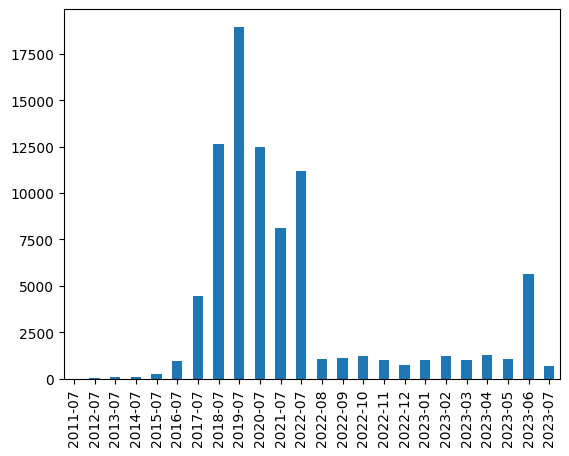
\includegraphics[width=0.75\textwidth]{figs/exploratoria/distribuicao_ano_mes_avaliacao.png}
	\caption{Distribuição do número de avaliação por mês e ano}
	\label{img:dist_ano_mes_avaliacao}
\end{figure}

Tratamos então os dados de avaliações e agora possuímos a nova coluna \textit{mes\_ano\_avaliacao}, na Figura~\ref{img:dist_ano_mes_avaliacao}, nota-se um comportamento estranho com a ausência de diversos meses por ano, durante o período de 2011 até 2021 temos o registro de apenas avaliações no mês 7, este comportamento é devido ao formato de data relativa utilizada pelo \textit{Google Maps} ao expor suas avaliações, não foi possível identificar uma forma de adquirir o tempo definitivo de quando a avaliação foi publicada.

Por este motivo ao se utilizar a data relativa passamos a ter dificuldade com as avaliações mais antigas, e conseguimos apenas identificar o ano no qual a avaliação foi publicada, as avaliações com menos de um ano de diferença da data de recuperação e utilizando este \textit{script} poderiam ser utilizadas em uma análise mais detalhada em relação ao período, porém esta não será a estratégia adotada e optaremos por restringir a análise de maneira que as avaliações serão agrupadas em períodos anuais, representando assim o ano de publicação de cada avaliação.

\begin{table}[]
	\centering
	\begin{tabular}{|l|l|}
		\hline
		\textbf{Ano} & \textbf{Quantidade} \\\hline
		2023         & 11925               \\
		2022         & 16364               \\
		2021         & 8104                \\
		2020         & 12489               \\
		2019         & 18963               \\
		2018         & 12625               \\
		2017         & 4426                \\
		2016         & 940                 \\
		2015         & 247                 \\
		2014         & 106                 \\
		2013         & 88                  \\
		2011         & 5                   \\
		2012         & 9                   \\
		\hline
	\end{tabular}%
	\caption{Quantidade de avaliações obtidas por ano}
	\label{table:review_per_year}
\end{table}

Considerando todas as avaliações obtidas podemos observar na Tabela~\ref{table:review_per_year} que temos uma discrepância na quantidade e é perceptível a divisão no período de 2017/2018.

E dessa forma foi definido que serão utilizadas avaliações posteriores a 2018.

Resultando um código conforme abaixo:

\lstinputlisting[language=Python,caption=Filtros aplicados ao dataset de avalições]{extras/code/review_filter.py}

Considerando todas as avaliações obtidas, temos:

\begin{itemize}
	\item 80470(93.25\%) enviadas depois de 2017 e 5821(6.75\%) enviadas em 2017, ou antes
	\item 56893(65.93\%) com texto e 3 ou mais caracteres, 29386(34.05\%) sem texto e 12(0.01\%) avaliações com 1 ou 2 caracteres
	\item 4184(4.85\%) avaliações traduzidas
\end{itemize}

Agora estamos considerando apenas avaliações que serão utilizadas na análise, a distribuição das notas atribuídas individualmente a cada avaliação pode ser consultada na Figura~\ref{img:dist_review_rating}. É fácil notar que a grande maioria das avaliações registradas, mais especificamente 38347 (77,91\%), possui a maior nota atribuída, de valor 5, o que nos leva a acreditar que na maioria das avaliações o sentimento geral que deve ser identificado será positivo.

\begin{figure}
	\centering
	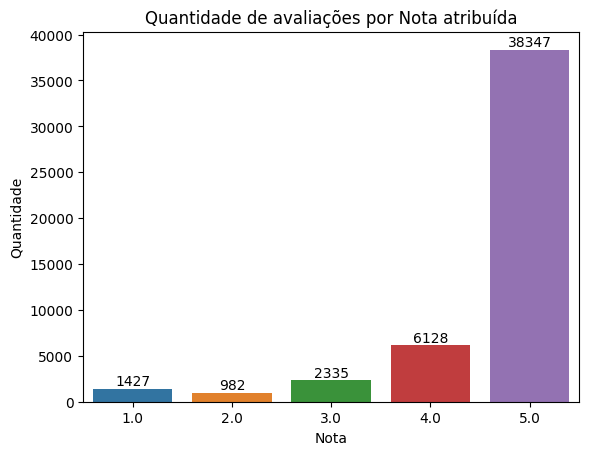
\includegraphics[width=0.75\textwidth]{figs/exploratoria/quantidade_avaliacao_nota_atribuida.png}
	\caption{Quantidade de avaliações por nota atribuída}
	\label{img:dist_review_rating}
\end{figure}

Este comportamento de distribuição desigual das notas ainda é perceptível também quando olhamos para as avaliações agrupadas por ano de submissão, como se pode notar na Figura~\ref{img:dist_review_rating_per_year}. Podemos também observar na Figura~\ref{img:dist_review_rating_per_year} a evolução em quantidade numérica durante o tempo, podendo notar uma quebra de tendência no crescimento pós 2019, nos anos de 2020 e 2021, provavelmente causado pelo confinamento decorrente da COVID-19~\cite{Guardia2022} e já pós-flexibilização do confinamento, 2022, visualizamos um aumento expressivo no número de avaliações, levando ainda em consideração que temos apenas 6 meses de avaliação em 2023 então seguiremos possivelmente com a tendência de aumento de número de avaliações ano após ano provavelmente 2023 será o ano com maior número de avaliações.

\begin{figure}
	\centering
	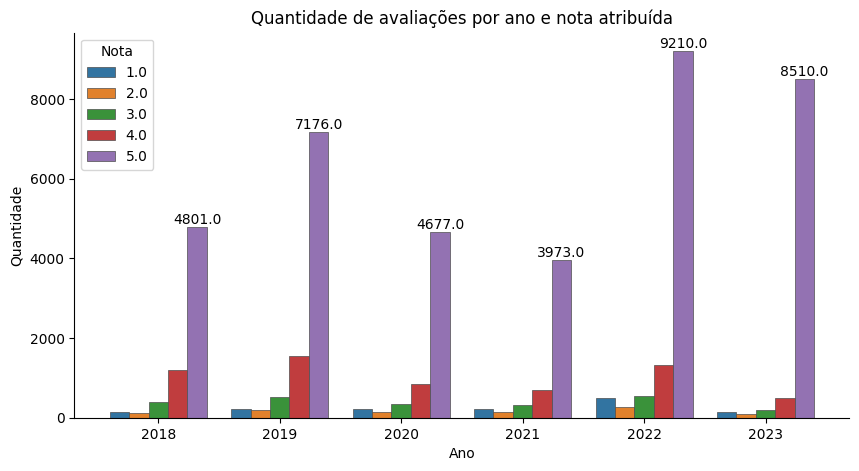
\includegraphics[width=1\textwidth]{figs/exploratoria/quantidade_avaliacao_nota_atribuida_ano.png}
	\caption{Quantidade de avaliações por ano e nota atribuída}
	\label{img:dist_review_rating_per_year}
\end{figure}

Com a Figura~\ref{img:relplot_ano_rating} podemos notar que a variação da nota atribuída tende a diminuir conforme o tempo passa, pois a quantidade de notas maiores é cresce de forma desproporcional se comparado com as avaliações com notas baixas, como observado na Figura~\ref{img:dist_review_rating_per_year}.

% \begin{figure}
% 	\centering
% 	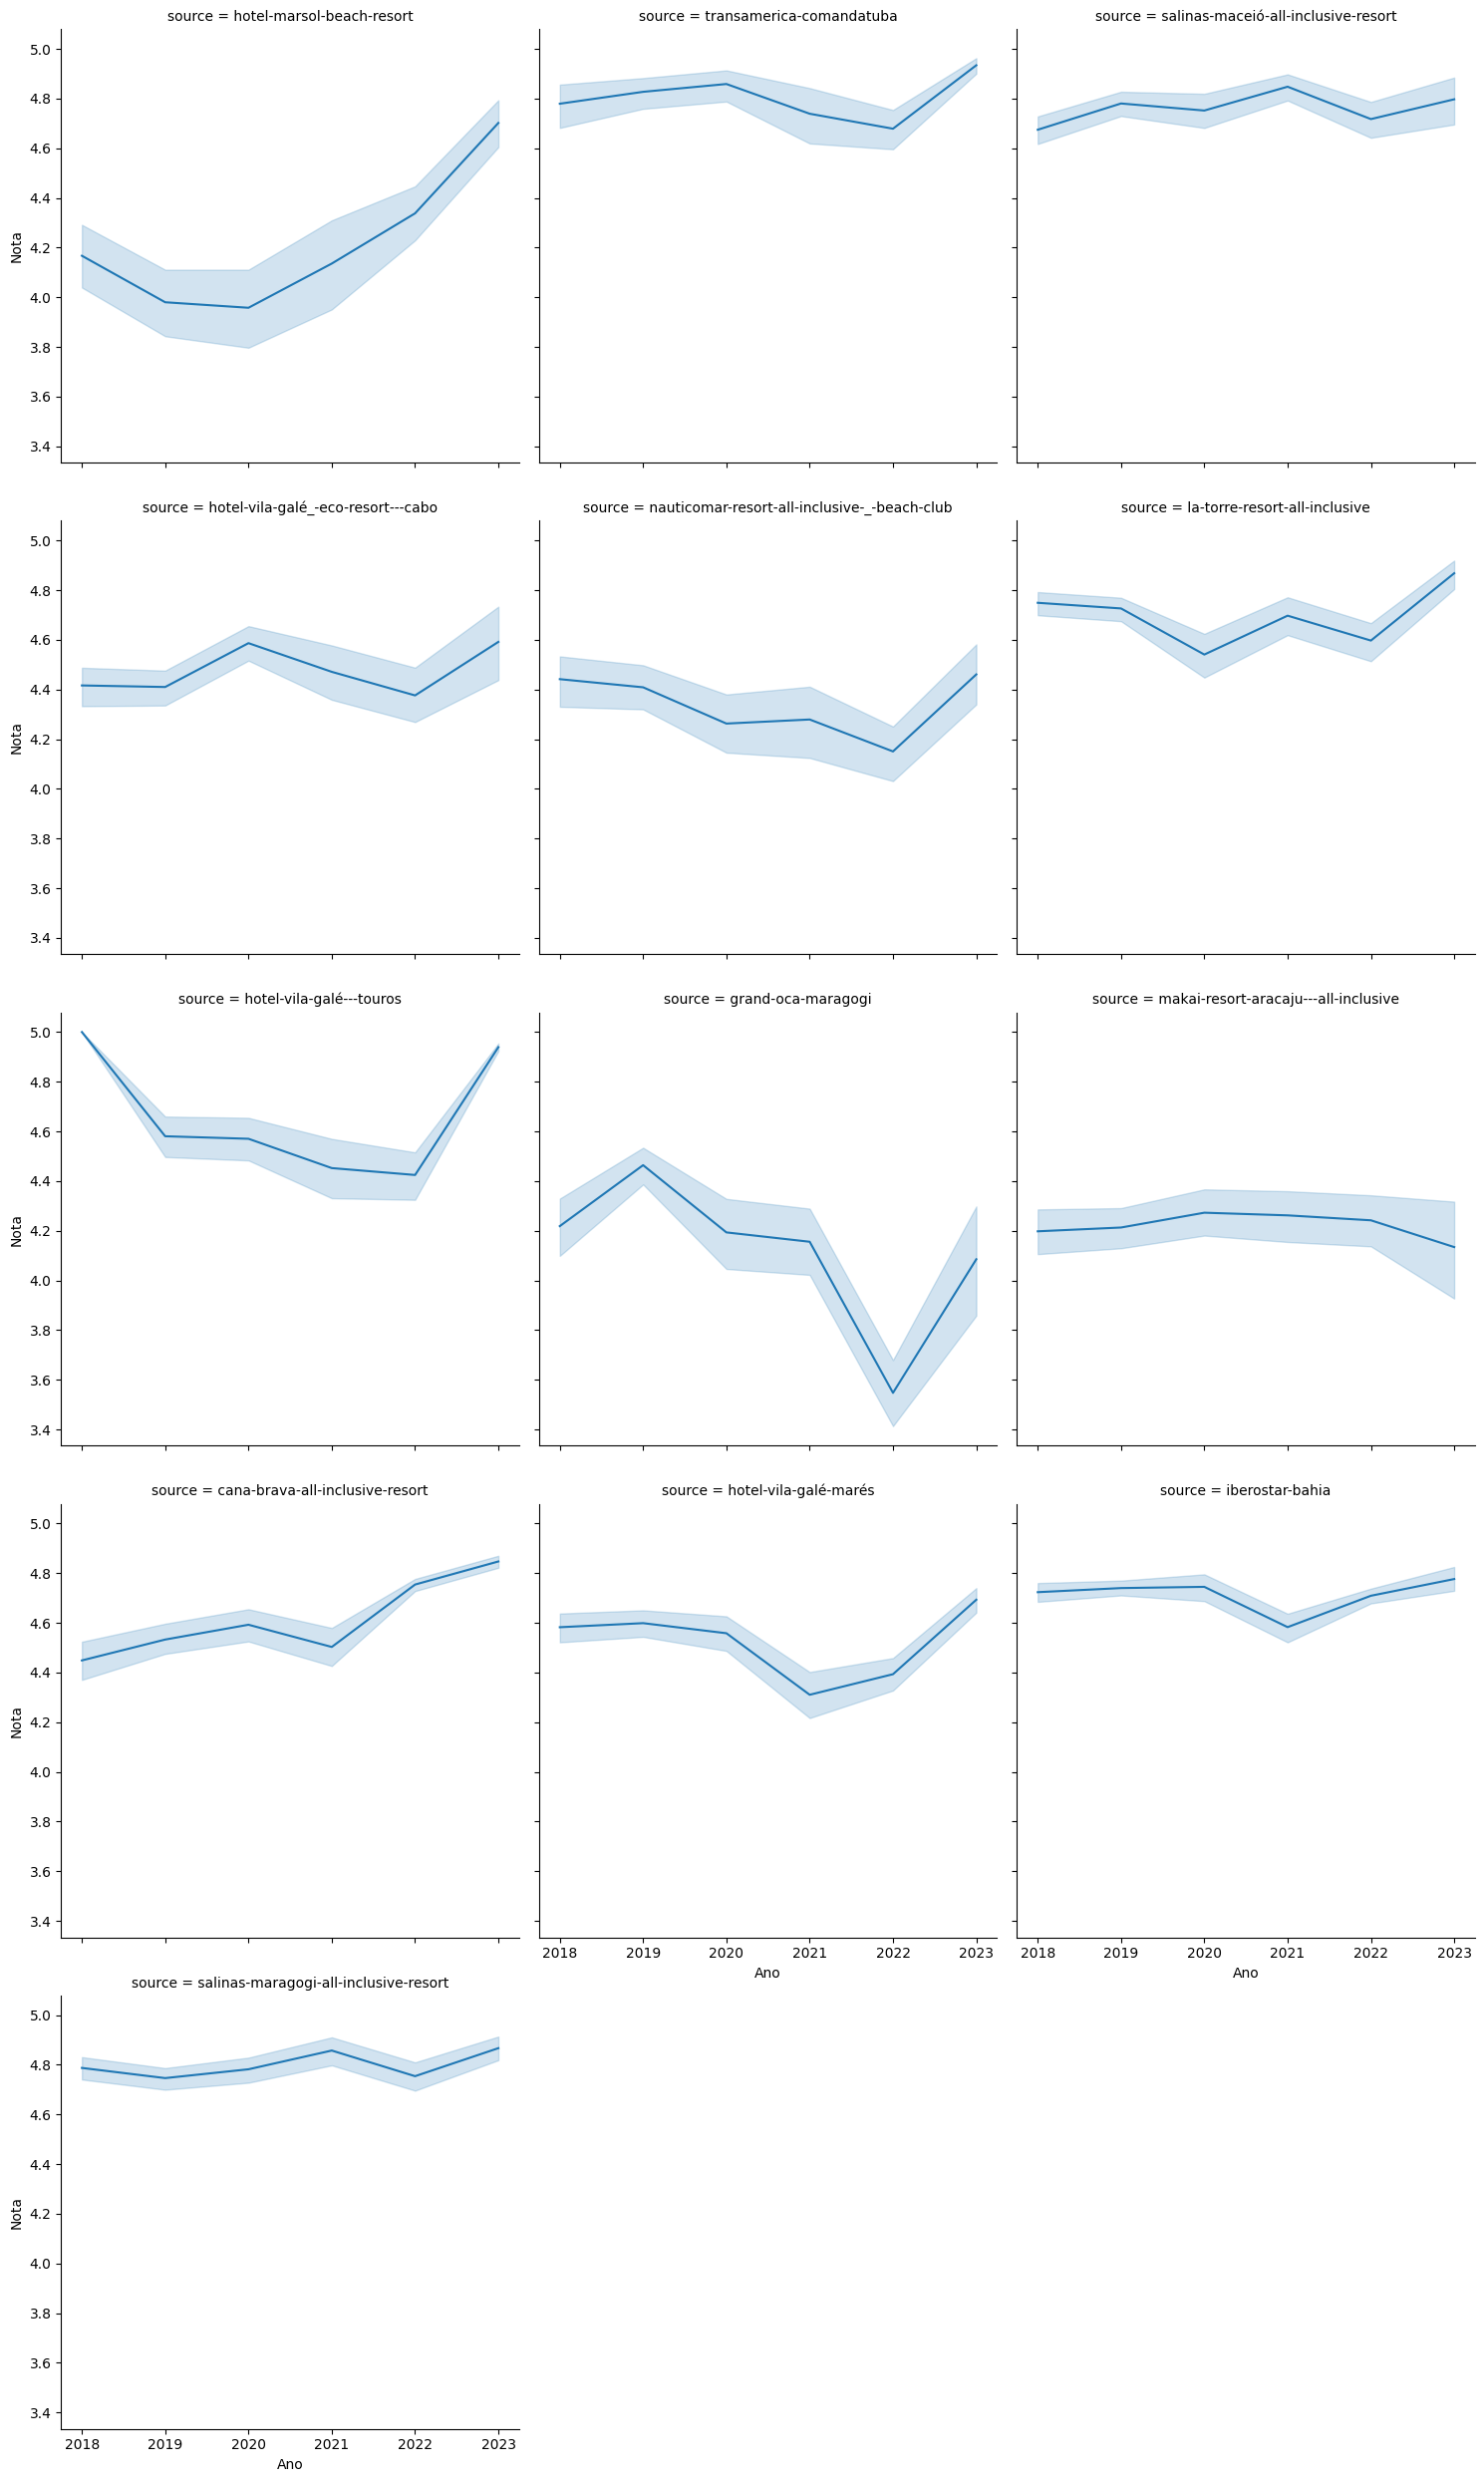
\includegraphics[width=1\textwidth]{figs/exploratoria/relplot_ano_rating_source.png}
% 	\caption{Variação da nota atribuída ao longo dos anos por hotel}
% 	\label{img:relplot_ano_rating_source}
% \end{figure}

\begin{table}[]
	\centering
	\begin{tabular}{|p{5cm}|l|l|l|l|}
		\hline
		\textbf{Hotel}                                      &
		\textbf{Não vazio}                                  &
		\textbf{Com texto}                                  &
		\textbf{Traduzido}                                  &
		\textbf{Públicos em +2017}                            \\
		\hline
		\textbf{Cana Brava All Inclusive Resort}            &
		8583                                                &
		8581                                                &
		141                                                 &
		10656                                                 \\
		\hline
		\textbf{Grand Oca Maragogi}                         &
		2948                                                &
		2947                                                &
		542                                                 &
		4297                                                  \\
		\hline
		\textbf{Hotel Marsol Beach Resort}                  &
		2150                                                &
		2150                                                &
		162                                                 &
		3128                                                  \\
		\hline
		\textbf{Hotel Vila Galé - Touros}                   &
		4481                                                &
		4480                                                &
		111                                                 &
		5802                                                  \\
		\hline
		\textbf{Hotel Vila Galé - Marés}                    &
		5723                                                &
		5721                                                &
		315                                                 &
		7981                                                  \\
		\hline
		\textbf{Hotel Vila Galé Eco Resort - Cabo}          &
		3219                                                &
		3217                                                &
		183                                                 &
		4934                                                  \\
		\hline
		\textbf{Iberostar Bahia}                            &
		10587                                               &
		10586                                               &
		1464                                                &
		14848                                                 \\
		\hline
		\textbf{La Torre Resort - All Inclusive}            &
		3847                                                &
		3847                                                &
		496                                                 &
		5722                                                  \\
		\hline
		\textbf{Makai Resort Aracaju - All Inclusive}       &
		3180                                                &
		3180                                                &
		84                                                  &
		4917                                                  \\
		\hline
		\textbf{Nauticomar Resort All Inclusive Beach Club} &
		2630                                                &
		2628                                                &
		228                                                 &
		3938                                                  \\
		\hline
		\textbf{Salinas Maceió All Inclusive Resort}        &
		2836                                                &
		2836                                                &
		168                                                 &
		4497                                                  \\
		\hline
		\textbf{Salinas Maragogi All Inclusive Resort}      &
		4572                                                &
		4572                                                &
		203                                                 &
		6700                                                  \\
		\hline
		\textbf{Transamerica Comandatuba}                   &
		2149                                                &
		2148                                                &
		87                                                  &
		3050                                                  \\ \hline
	\end{tabular}
	\caption{Quantidade de avaliações em cada filtro pro hotél}
	\label{table:qtd_review_filtro}
\end{table}

\begin{table}[h]
	\centering
	\begin{tabular}{|c|crrrrr|}
		\hline
		\multicolumn{1}{|c|}{\multirow{2}{*}{\textbf{Estado}}} &
		\multicolumn{2}{c|}{\textbf{analisar}}                 &
		\multicolumn{3}{c|}{\textbf{nota}}                     &
		\multicolumn{1}{c|}{\textbf{estrelas}}                                                                            \\ \cline{2-7}
		\multicolumn{1}{|l|}{}                                 &
		\multicolumn{1}{c}{\textbf{rotulo}}                    &
		\multicolumn{1}{c|}{\textbf{quantidade}}               &
		\multicolumn{1}{c}{\textbf{média}}                     &
		\multicolumn{1}{c}{\textbf{min}}                       &
		\multicolumn{1}{c|}{\textbf{max}}                      &
		\multicolumn{1}{c|}{\textbf{média}}                                                                               \\ \hline
		\multirow{2}{*}{\textbf{AL}}                           & \textbf{False} & 8106  & 4.623896 & 4.3 & 4.8 & 4.735998 \\
		                                                       & \textbf{True}  & 8668  & 4.643205 & 4.3 & 4.8 & 4.706853 \\ \hline
		\multirow{2}{*}{\textbf{BA}}                           & \textbf{False} & 20970 & 4.617740 & 4.3 & 4.8 & 4.542680 \\
		                                                       & \textbf{True}  & 28727 & 4.613016 & 4.3 & 4.8 & 4.467017 \\ \hline
		\multirow{2}{*}{\textbf{PE}}                           & \textbf{False} & 2645  & 4.500000 & 4.5 & 4.5 & 5.000000 \\
		                                                       & \textbf{True}  & 2746  & 4.500000 & 4.5 & 4.5 & 5.000000 \\ \hline
		\multirow{2}{*}{\textbf{RN}}                           & \textbf{False} & 2903  & 4.397451 & 4.2 & 4.6 & 4.493627 \\
		                                                       & \textbf{True}  & 6232  & 4.480424 & 4.2 & 4.6 & 4.701059 \\ \hline
		\multirow{2}{*}{\textbf{SE}}                           & \textbf{False} & 2448  & 4.300000 & 4.3 & 4.3 & 4.000000 \\
		                                                       & \textbf{True}  & 2846  & 4.300000 & 4.3 & 4.3 & 4.000000 \\ \hline
	\end{tabular}\caption{Quantidade de avaliações por estado e por rotulo -- indicando o que será e o que não será analisado}
	\label{table:distribuicao_review_por_estado}
\end{table}

E dentre todas as avaliações obtidas após aplicar o filtro de período utilizaremos para a análise o total de 49219(57.04\%) e 37072(42.96\%) foram ignoradas. Assim as avaliações que foram consideradas estão então distribuídas conforme a Tabela~\ref{table:distribuicao_review_per_year}.

\begin{table}[h]
	\centering
	\begin{tabular}{|l|l|}
		\hline
		\textbf{Ano} & \textbf{Quantidade} \\\hline
		2023         & 9444                \\
		2022         & 11866               \\
		2021         & 5350                \\
		2020         & 6236                \\
		2019         & 9645                \\
		2018         & 6678                \\
		\hline
	\end{tabular}
	\caption{Quantidade de avaliações por ano após filtro}
	\label{table:distribuicao_review_per_year}
\end{table}

% TODO

\begin{table}[h]
	\centering
	\begin{tabular}{|c|c|r|r|}
		\hline
		\multicolumn{1}{|r|}{\textbf{Hotel}}                                    &
		\multicolumn{1}{r|}{\textbf{Analisar?}}                                 &
		\textbf{Quantidade}                                                     &
		\textbf{\%}                                                               \\ \hline
		\multirow{2}{*}{\textbf{Cana Brava All Inclusive Resort}}               &
		False                                                                   &
		3028                                                                    &
		27.16                                                                     \\ \cline{2-4}
		                                                                        &
		True                                                                    &
		8119                                                                    &
		72.84                                                                     \\ \hline
		\multirow{2}{*}{\textbf{Grand Oca Maragogi}}                            &
		False                                                                   &
		2427                                                                    &
		52.34                                                                     \\ \cline{2-4}
		                                                                        &
		True                                                                    &
		2210                                                                    &
		47.66                                                                     \\ \hline
		\multirow{2}{*}{\textbf{Hotel Marsol Beach Resort}}                     &
		False                                                                   &
		1470                                                                    &
		44.10                                                                     \\ \cline{2-4}
		                                                                        &
		True                                                                    &
		1863                                                                    &
		55.90                                                                     \\ \hline
		\multirow{2}{*}{\textbf{Hotel Vila Galé - Touros}}                      &
		False                                                                   &
		1433                                                                    &
		24.70                                                                     \\ \cline{2-4}
		                                                                        &
		True                                                                    &
		4369                                                                    &
		75.30                                                                     \\ \hline
		\multirow{2}{*}{\textbf{Hotel Vila Galé - Marés}}                       &
		False                                                                   &
		3550                                                                    &
		41.36                                                                     \\ \cline{2-4}
		                                                                        &
		True                                                                    &
		5033                                                                    &
		58.64                                                                     \\ \hline
		\multirow{2}{*}{\textbf{Hotel Vila Galé: Eco Resort - Cabo}}            &
		False                                                                   &
		2645                                                                    &
		49.06                                                                     \\ \cline{2-4}
		                                                                        &
		True                                                                    &
		2746                                                                    &
		50.94                                                                     \\ \hline
		\multirow{2}{*}{\textbf{Iberostar Bahia}}                               &
		False                                                                   &
		7830                                                                    &
		48.29                                                                     \\ \cline{2-4}
		                                                                        &
		True                                                                    &
		8383                                                                    &
		51.71                                                                     \\ \hline
		\multirow{2}{*}{\textbf{La Torre Resort All Inclusive}}                 &
		False                                                                   &
		3164                                                                    &
		50.84                                                                     \\ \cline{2-4}
		                                                                        &
		True                                                                    &
		3060                                                                    &
		49.16                                                                     \\ \hline
		\multirow{2}{*}{\textbf{Makai Resort Aracaju - All Inclusive}}          &
		False                                                                   &
		2448                                                                    &
		46.24                                                                     \\ \cline{2-4}
		                                                                        &
		True                                                                    &
		2846                                                                    &
		53.76                                                                     \\ \hline
		\multirow{2}{*}{\textbf{Nauticomar Resort All Inclusive \& Beach Club}} &
		False                                                                   &
		2104                                                                    &
		49.03                                                                     \\ \cline{2-4}
		                                                                        &
		True                                                                    &
		2187                                                                    &
		50.97                                                                     \\ \hline
		\multirow{2}{*}{\textbf{Salinas Maceió All Inclusive Resort}}           &
		False                                                                   &
		2140                                                                    &
		45.72                                                                     \\ \cline{2-4}
		                                                                        &
		True                                                                    &
		2541                                                                    &
		54.28                                                                     \\ \hline
		\multirow{2}{*}{\textbf{Salinas Maragogi All Inclusive Resort}}         &
		False                                                                   &
		3539                                                                    &
		47.46                                                                     \\ \cline{2-4}
		                                                                        &
		True                                                                    &
		3917                                                                    &
		52.54                                                                     \\ \hline
		\multirow{2}{*}{\textbf{Transamerica Comandatuba}}                      &
		False                                                                   &
		1294                                                                    &
		39.95                                                                     \\ \cline{2-4}
		                                                                        &
		True                                                                    &
		1945                                                                    &
		60.05                                                                     \\ \hline
	\end{tabular}
	\caption{Lista de quantidade de avaliações analisadas e descartadas por hotel}
	\label{tab:lista_review_hoteis}
\end{table}

Após devido tratamento das avaliações conseguimos obter as nuvens de palavras considerando todas as palavras na Figura~\ref{img:wordcloud_geral}, onde podemos notar como alguns dos destaques quarto, piscina, praia, restaurante, como sendo as palavras com maior frequência nas avaliações.

\begin{figure}
	\centering
	\begin{minipage}{0.45\textwidth}
		\centering
		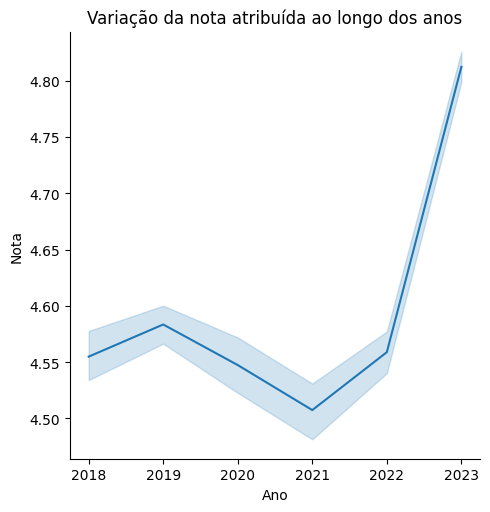
\includegraphics[width=1\textwidth]{figs/exploratoria/relplot_ano_rating.png}
		\caption{Variação da nota atribuída ao longo dos anos}
		\label{img:relplot_ano_rating}
	\end{minipage}\hfill
	\begin{minipage}{0.45\textwidth}
		\centering
		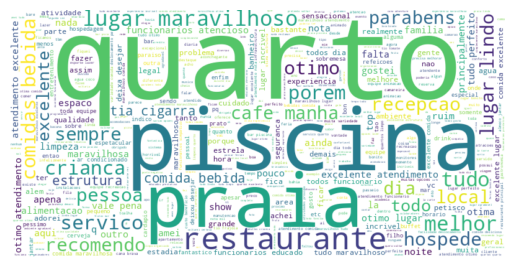
\includegraphics[width=1\textwidth]{figs/exploratoria/wordcloud_geral.png}
		\caption{Wordcloud sem \textit{stop words}}
		\label{img:wordcloud_geral}
	\end{minipage}
\end{figure}

Já considerando a nuvem de palavras filtrando apenas por adjetivos teremos então na Figura~\ref{img:wordcloud_adjetivos} que tem como alguns dos destaques palavras como sensacional, excelente, especial, local, top, ótimo, nota.

E por último observamos a nuvem de palavras levando em consideração apenas os substantivos na Figura~\ref{img:wordcloud_substantivos}, que como destaque podemos citar funcionário, piscina, quarto, praia.

\begin{figure}
	\centering
	\begin{minipage}{0.45\textwidth}
		\centering
		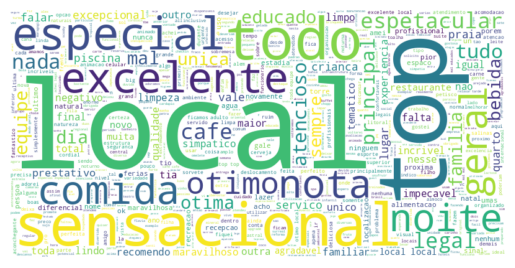
\includegraphics[width=1\textwidth]{figs/exploratoria/wordcloud_adjetivos.png}
		\caption{Wordcloud de Adjetivos}
		\label{img:wordcloud_adjetivos}
	\end{minipage}
	\begin{minipage}{0.45\textwidth}
		\centering
		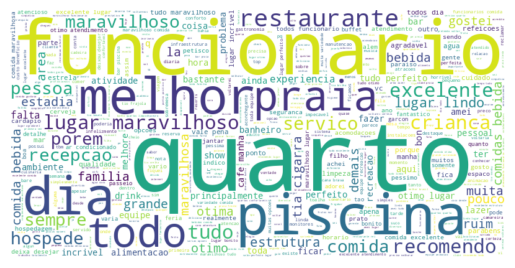
\includegraphics[width=1\textwidth]{figs/exploratoria/wordcloud_substantivos.png}
		\caption{Wordcloud de substantivos}
		\label{img:wordcloud_substantivos}
	\end{minipage}
\end{figure}

Outra forma de análise é o agrupamento de \textit{tokens} em unigramas na Figura~\ref{img:unigramas}, bigramas na Figura~\ref{img:bigramas} e os trigramas na Figura~\ref{img:trigramas} presentes em todas as avaliações. E dessa forma temos exatamente a classificação de frequência dos \textit{tokens} no corpus de estudo.

Entre os unigramas, Figura~\ref{img:unigramas}, temos uma lista com alguns dos \textit{tokens} mais frequentes, alguns chegando a passar a contagem de utilização de mais de 10.000 vezes, como é o caso de lugar, sendo seguindo ainda que próximo por comida, excelente e atendimento, este ultimo com uma frequência próximo de 8500 vezes. Ainda em relação aos unigramas também podemos levar em consideração a sua frequência com a evolução do tempo na Figura~\ref{img:rank_unigramas}, e algo com grande destaque é a palavra lugar que está entre o top 10 entre todo o período da análise, flutuando entre as cinco primeiras posições, tio é um unigrama que merece atenção, por não aparecer na nuvem de palavras de unigramas, porém se faz presente no ranking se observarmos individualmente os anos ele aparece em décimo lugar no ano de 2022, indícios de uma possível atração local bem conhecida, substituindo então o unigrama 'praia', que se fazia presente no ranking até 2021 na nona colocação.

\begin{figure}
	\centering
	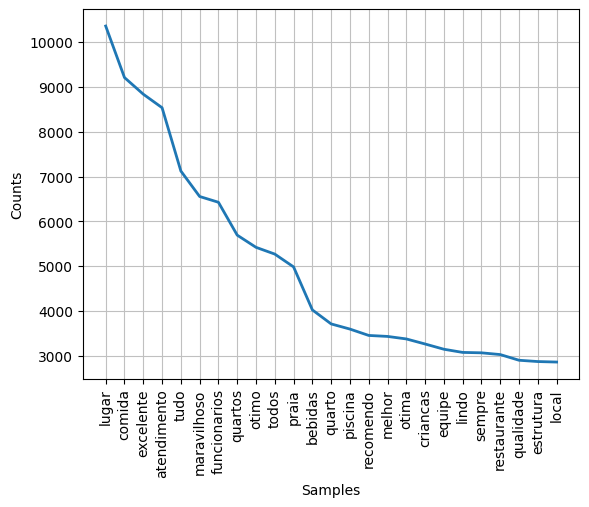
\includegraphics[width=.8\textwidth]{figs/exploratoria/unigramas.png}
	\caption{Unigramas}
	\label{img:unigramas}
\end{figure}

Considerando os bigramas na Figura~\ref{img:bigramas} a frequência diminui consideravelmente, pois aqui temos que a ordem importa e dessa forma o mais frequente fica próximo de 1700 vezes, sendo composto pela dupla 'lugar' e 'maravilhoso', seguido pelo segundo colocado, bem próximo de 1400 vezes, sendo 'comida' e 'boa', onde podemos observar a grande frequência de palavras positivas, por conta dos adjetivos positivos.

\begin{figure}[!h]
	\centering
	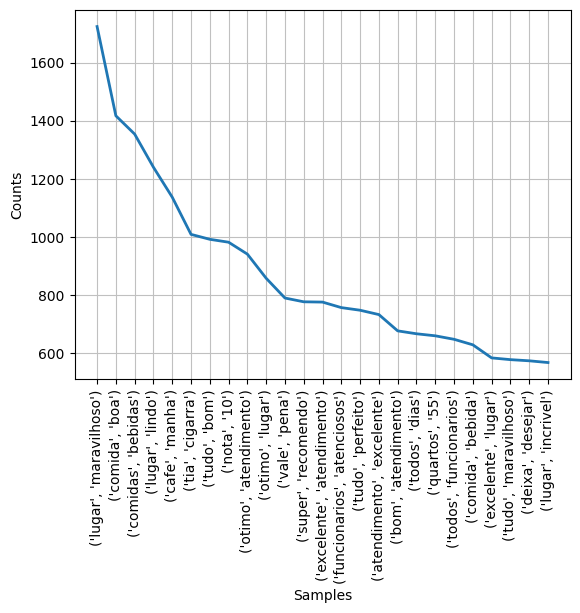
\includegraphics[width=.8\textwidth]{figs/exploratoria/bigramas.png}
	\caption{Bigramas}
	\label{img:bigramas}
\end{figure}

Para destaque entre os trigramas na Figura~\ref{img:trigramas} a frequência diminui ainda mais e como destaque temos um que supera a contagem de 250 vezes, sendo 'facilidade', 'deslocamento' e 'pe', o que nos indica que existe pelo menos um hotel que possui uma boa localização para ser possível se deslocar até uma atração popular do local a pé, seguido de 'atendimento', 'nota' e '10' que indica que para as pessoas que avaliaram o atendimento da rede de hotéis ainda é algo importante e que deve ser levado em consideração caso a rede tenha interesse em ter ou manter um conceito positivo entre seus clientes.

\begin{figure}
	\centering
	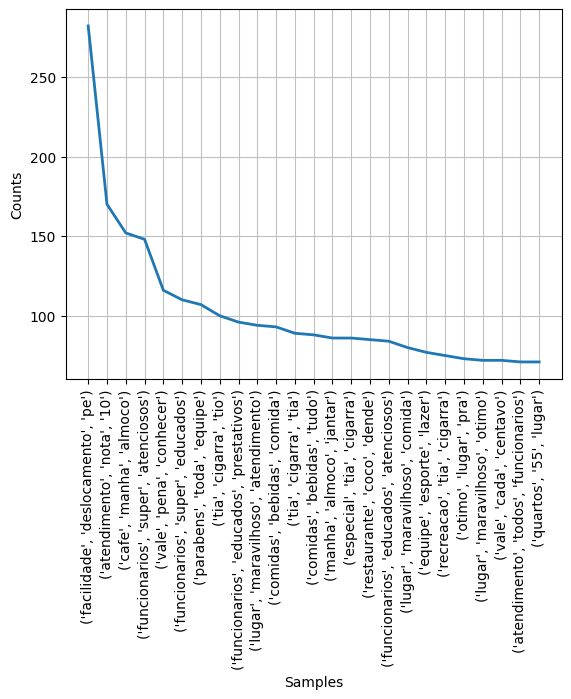
\includegraphics[width=.8\textwidth]{figs/exploratoria/trigramas.png}
	\caption{Trigramas}
	\label{img:trigramas}
\end{figure}

\begin{figure}
	\centering
	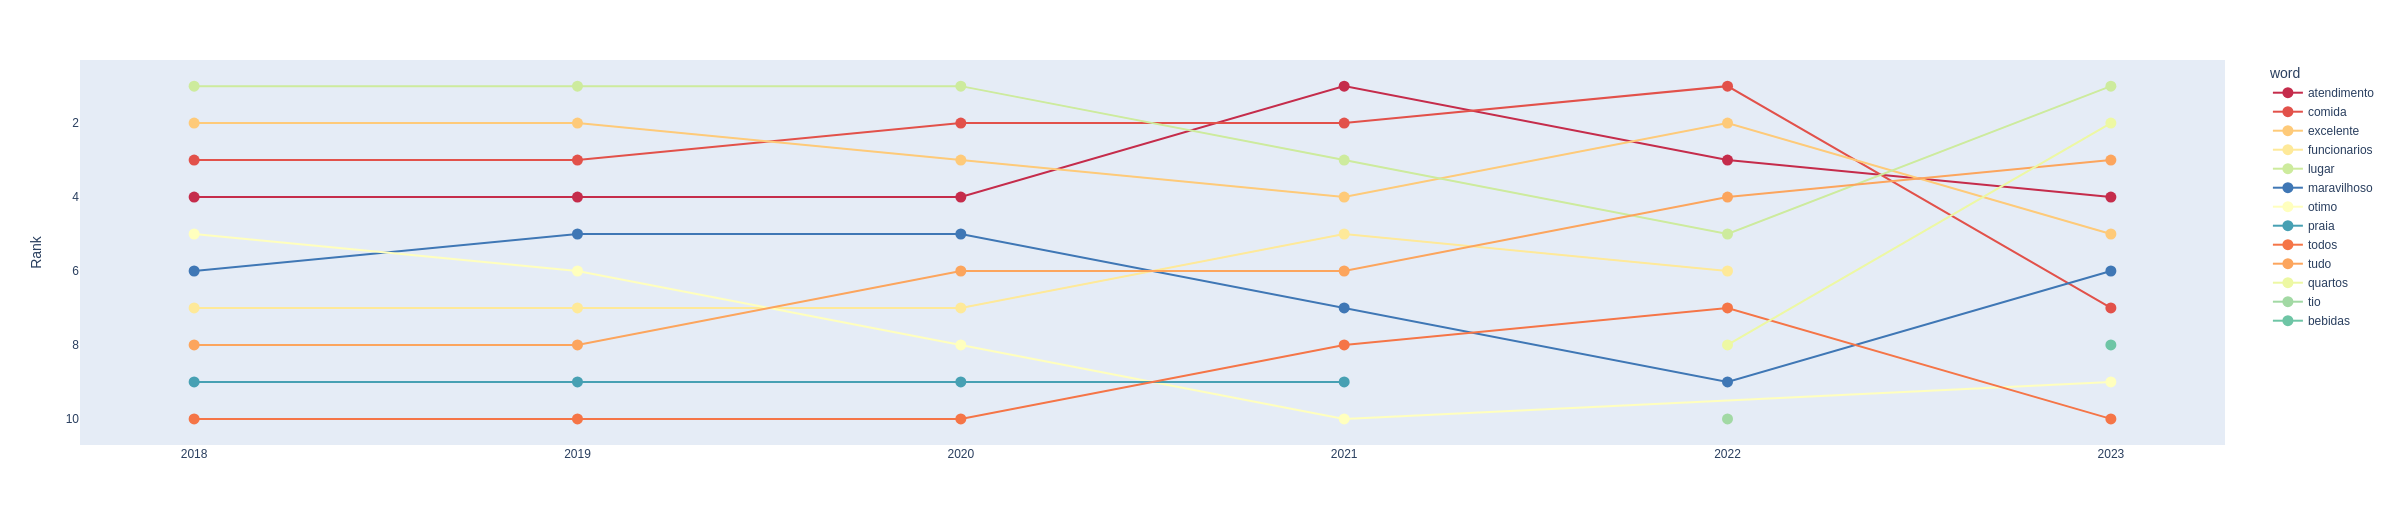
\includegraphics[width=1\textwidth]{figs/exploratoria/ranking_unigramas_por_ano.png}
	\caption{Ranking de unigramas por ano}
	\label{img:rank_unigramas}
\end{figure}

\section{Análise de Sentimentos Temporal}
\label{cap:resultados:sec:analise_sentimento}

\subsection[BERT]{BERT}
\label{sec:resultados:subsec:bert}

O tempo de execução médio, após 5 execuções cada, para que a análise de todo o corpus fosse realizada, foi o seguinte:

\begin{itemize}
	\item philschmid/distilbert-base-multilingual-cased-sentiment: 3min e 37s
	\item lxyuan/distilbert-base-multilingual-cased-sentiments-student: 3min e 36s
	\item citizenlab/twitter-xlm-roberta-base-sentiment-finetunned: 6min e 54s
	\item cardiffnlp/twitter-xlm-roberta-base-sentiment: 6min e 44s
	\item ramonmedeiro1/bertimbau-products-reviews-pt-br: 6min e 59s
\end{itemize}

Considerando apenas os \textit{BERTs} notamos um desempenho com relação à velocidade de execução bem interessante, levando em consideração o ambiente de execução que estamos utilizando para realizar os testes que possui um poder computacional razoável para os tempos modernos.

Após realizar o tratamento e levar em consideração o \textit{score} mais alto, temos quase 86\% das avaliações identificadas com o sentimento Positivo, em números absolutos 42078 avaliações, pouco mais de 6\% contendo sentimento Neutro e pouco mais de 8\% com sentimento negativo, como podemos observar na Figura~\ref{img:sentimento_bert}.

\begin{figure}
	\centering
	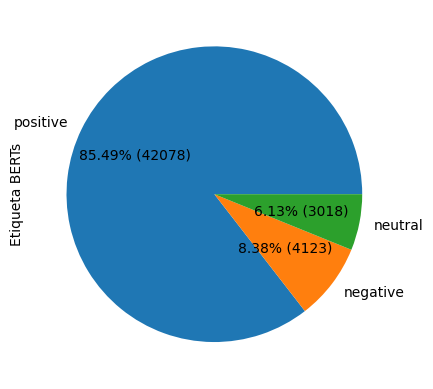
\includegraphics{figs/bert/distribuicao_pizza.png}
	\caption{\textit{BERTs} - Distribuição do sentimento das avaliações}
	\label{img:sentimento_bert}
\end{figure}

Como já era esperado, a grande maioria das avaliações foram classificadas como sendo avaliações com sentimento positivo, em todos os anos, como é possível ser observado na Figura~\ref{img:sentimento_timechart_bert}.

Também conseguimos notar que quanto maior a nota maior a quantidade de avaliações com sentimento positivo, sendo que as avaliações com notas 4 e 5 contém uma discrepância grande com relação à quantidade de avaliações com sentimento positivo contra a quantidade de avaliações com sentimento neutro ou negativo, já as avaliações com nota 3 possuem uma distribuição mais equivalente e as avaliações com notas 1 e 2 com o sentimento negativo tendo grande destaque em relação às avaliações etiquetadas como neutro ou positivo, como é possível ser observado na Figura~\ref{img:sentimento_nota_bert}, que indica que os usuários tendem a dar uma nota mais elevada quando escrevem uma avaliação com um sentimento mais positivo.

\begin{figure}
	\centering
	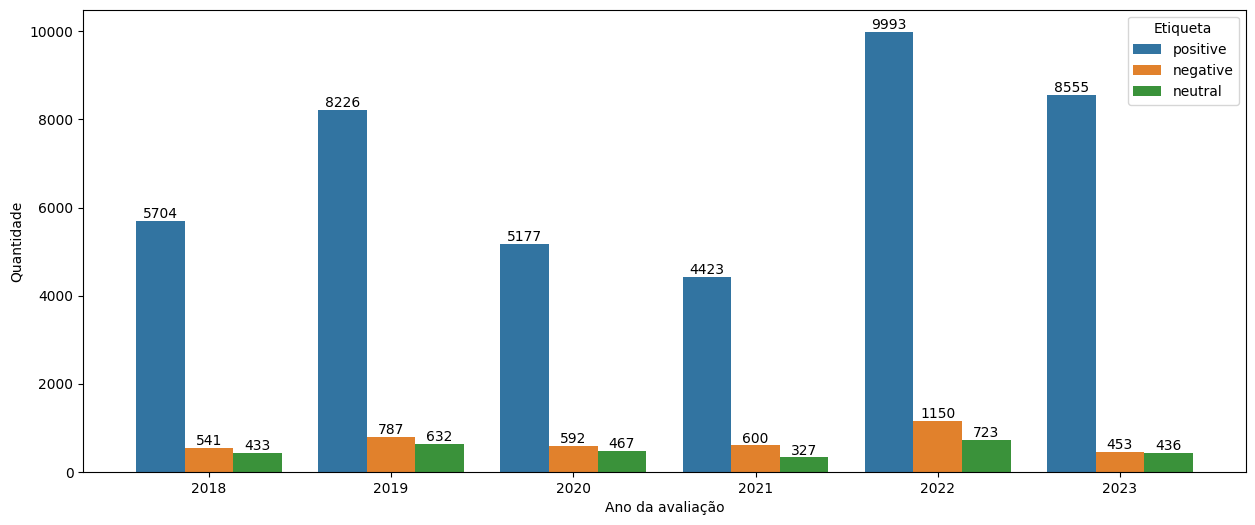
\includegraphics[width=1\textwidth]{figs/bert/sentimento_ano.png}
	\caption{\textit{BERTs} - Sentimento das avaliações por ano}
	\label{img:sentimento_timechart_bert}
\end{figure}

\begin{figure}
	\centering
	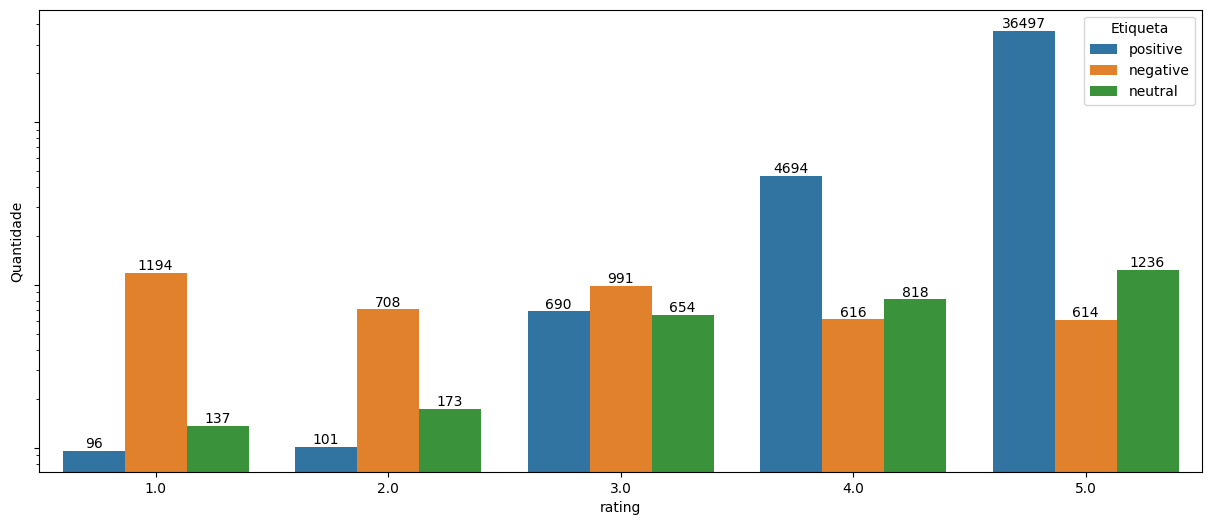
\includegraphics[width=1\textwidth]{figs/bert/sentimento_nota.png}
	\caption{\textit{BERTs} - Sentimento das avaliações por nota}
	\label{img:sentimento_nota_bert}
\end{figure}

Porém, avaliando de forma individual cada um dos modelos, podemos notar uma grande discrepância entre eles, com a afinação mais eficiente para esse corpus sendo o do \textit{citizenlab}, considerando que eficiência aqui representa a maior número de avaliações classificadas com \textit{score} superior aos outros, como notamos na Figura~\ref{img:rinha_de_berts}, modelo esse que levou menos de 7 minutos para executar e classificar todo o corpus, seguido pelo \textit{philschmid} que levou cerca de 3 minutos e meio na média.

\begin{figure}
	\centering
	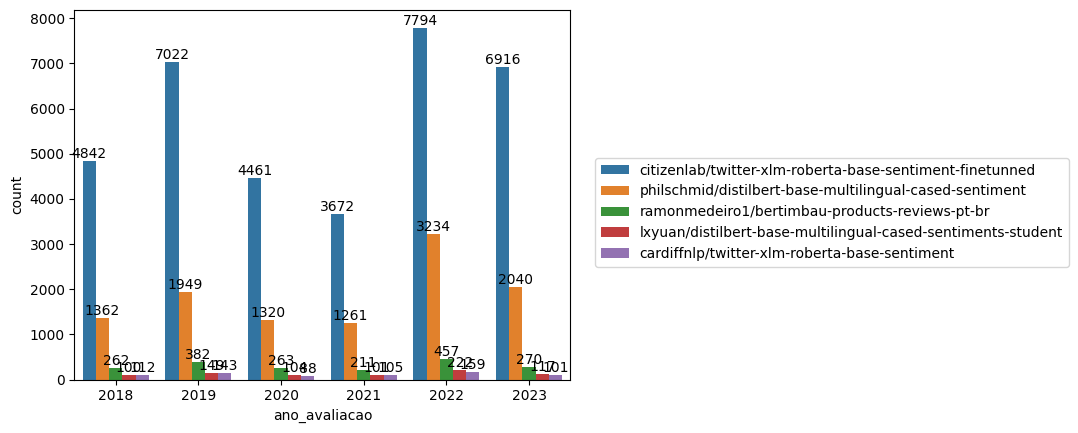
\includegraphics[width=1\textwidth]{figs/bert/desempenho_berts.png}
	\caption{\textit{BERTs} - Quantidade de avaliações com maior \textit{score} por ano}
	\label{img:rinha_de_berts}
\end{figure}

Nas Figuras~\ref{img:sentimento_phil} e~\ref{img:sentimento_citizenlab} conseguimos visualizar a classificação atribuída de forma individual por ambos os modelos, a versão de \textit{philschmid} e \textit{citizenlab} respectivamente, com o \textit{citizenlab} classificando um número maior de sentimentos positivos, porém com um número de sentimentos neutros e negativos similar, o mesmo não acontece com \textit{philschmid} que tem um número maior de sentimentos neutros em comparação direta, porém da mesma forma um número de sentimento positivo maior e desigual.

\begin{figure}
	\centering
	\centering
	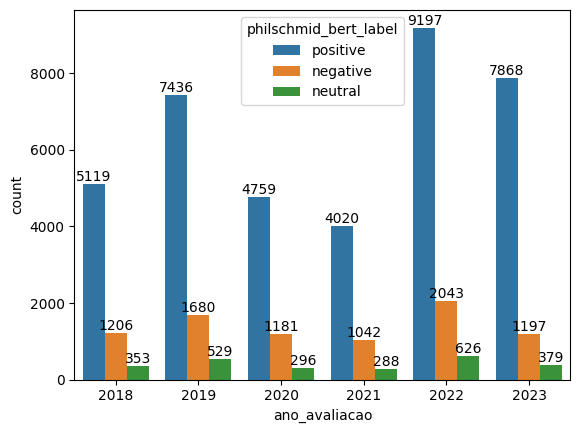
\includegraphics[width=1\textwidth]{figs/bert/classificacao_phil.png}
	\caption{\textit{BERT philschmid} - Sentimento das avaliações por ano}
	\label{img:sentimento_phil}
\end{figure}

\begin{figure}
	\centering
	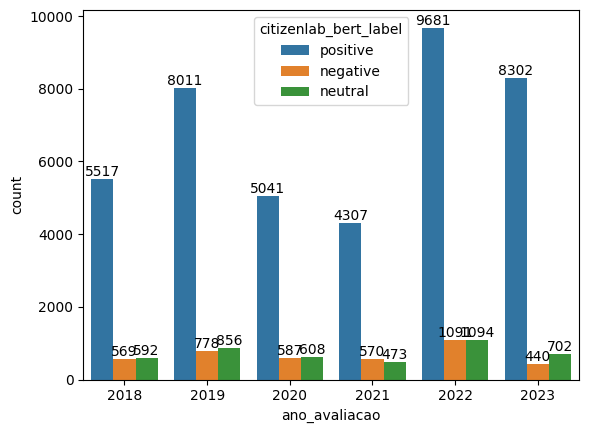
\includegraphics[width=1\textwidth]{figs/bert/classificacao_citizenlab.png}
	\caption{\textit{BERT citizenlab} - Sentimento das avaliações por ano}
	\label{img:sentimento_citizenlab}
\end{figure}


Todos os modelos \textit{BERTs} etiquetam as avaliações de forma aparentemente consistente, como era esperado, temos uma quantidade muito grande de avaliações com nota máxima, 5, e por esse motivo é esperado que o sentimento geral das avaliações de nota 4 ou 5 seja positivo, avaliações com nota 3 distribuição de sentimento mais uniforme e as notas 1 e 2 contendo uma quantidade maior de sentimento negativo.

Os resultados indicam que os modelos \textit{BERTs} concordam com o modelo \textit{GPT} em quase 89\% das avaliações, conforme Figura~\ref{img:bert_vs_gpt}, mostrando uma alta taxa de concordância geral entre os modelos na identificação de sentimentos. Essa elevada consistência sugere que ambos os modelos são eficazes na tarefa, especialmente em relação às avaliações positivas.

\begin{figure}
	\centering
	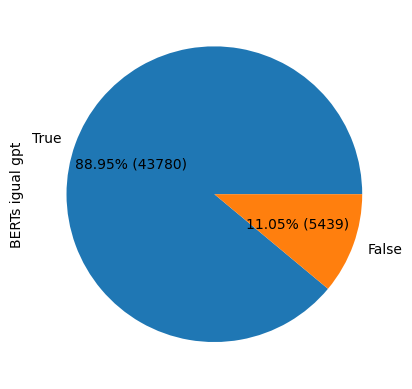
\includegraphics{figs/bert/vs_gpt.png}
	\caption{\textit{BERT} com sentimento igual ao GPT}
	\label{img:bert_vs_gpt}
\end{figure}

No entanto, a Figura~\ref{img:heat_bert_vs_gpt} revela áreas de discordância, principalmente nas avaliações negativas e neutras. Embora ambos os modelos concordem fortemente nas classificações positivas, com 40.224 avaliações coincidentes, há uma divergência considerável nas categorias negativas e neutras. Isso sugere que os modelos podem ter abordagens diferentes para sentimentos mais ambíguos ou menos claros, importante levar em consideração que o \textit{GPT} não conseguiu classificar todas as avaliações,falaremos mais sobre isso na seção do \textit{GPT}, em ~\ref{sec:resultados:subsec:gpt}.

\begin{figure}
	\centering
	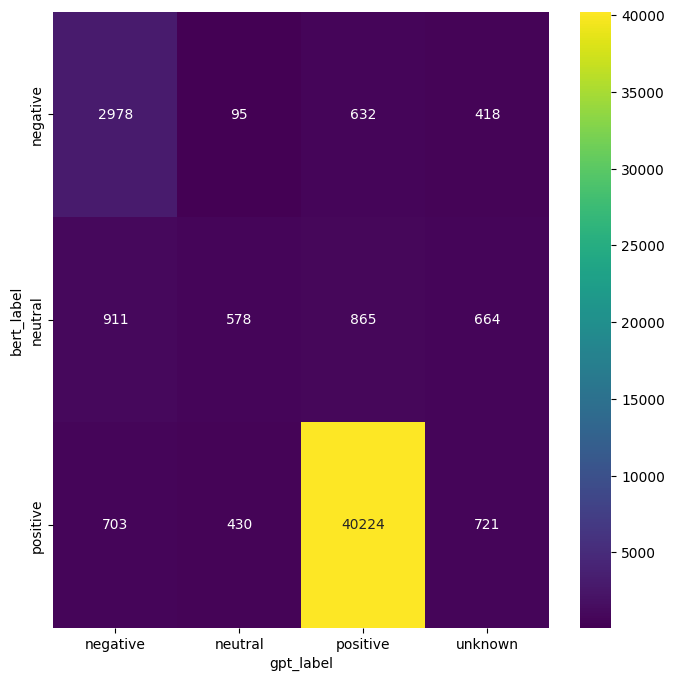
\includegraphics[width=.8\textwidth]{figs/bert/heat_vs_gpt.png}
	\caption{Distribuição de sentimento \textit{BERTs} comparado com GPT}
	\label{img:heat_bert_vs_gpt}
\end{figure}


\subsection{Vicuna}
\label{sec:resultados:subsec:vicuna}


O modelo \textit{Vicuna} demorou pouco mais do que 6 horas para realizar a tarefa de atribuição de etiqueta para cada uma das avaliações, o que é pode ser um ponto negativo dependendo do projeto que se está executando, ele demorou um tempo consideravelmente maior se comparado com os modelos \textit{BERTs} e para a tarefa proposta no trabalho ambos realizaram uma simular em termos de volume de etiquetas atribuídas para as avaliações, ambos reconheceram como sendo positivas a grande parte, mais de 86\% das avaliações, e o segundo maior grupo como sendo as avaliações negativas, como observado na Figura~\ref{img:vicuna_pizza_distribuicao}.

\begin{figure}
	\centering
	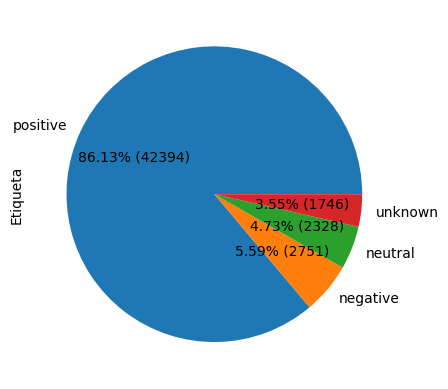
\includegraphics{figs/vicuna/distribuicao_pizza.png}
	\caption{\textit{Vicuna} - Distribuição do sentimento das avaliações}
	\label{img:vicuna_pizza_distribuicao}
\end{figure}

Continuamos aqui com o mesmo comportamento de quantidade de avaliações com sentimento positivo brutalmente maior se comparado com os outros sentimentos, porém também temos agora o cenário onde o modelo não conseguir realizar a tarefa com sucesso e atribuir uma etiqueta apropriada a avaliação, dessa forma elas foram etiquetadas com o valor \textit{UNKNOWN}, temos 1746(3.55\%) avaliações nesse estado, cenário que não temos com os modelos \textit{BERT}, que considerando a quantidade total de avaliações pode ser considerado um número baixo, porém se avaliarmos ano a ano, a quantidade de avaliações com esse valor de etiqueta acaba se tornando relevante, até mesmo em quantidade superiores aos outros sentimentos (neutro e negativo), como observado na Figura~\ref{img:vicuna_sentimento_ano}, mas mesmo assim o \textit{Vicuna} atribuiu algum sentimento para a maioria das avaliações, sendo o grupo de avaliações com problema na classificação o grupo com menor quantidade de avaliações.

\begin{figure}
	\centering
	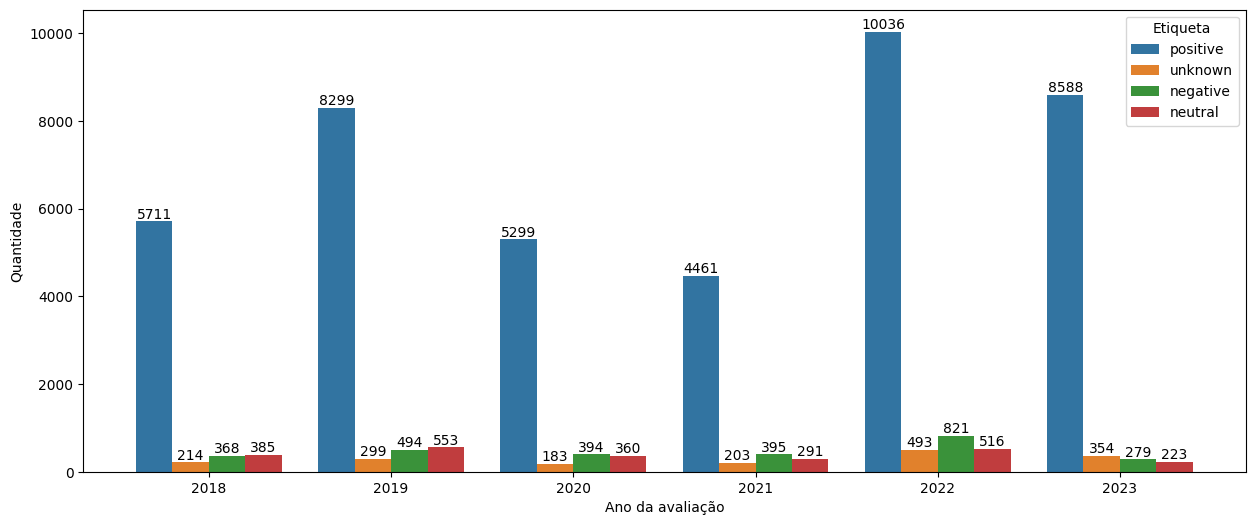
\includegraphics[width=1\textwidth]{figs/vicuna/sentimento_ano.png}
	\caption{\textit{Vicuna} - Sentimento das avaliações por ano}
	\label{img:vicuna_sentimento_ano}
\end{figure}

Olhando especificamente para a distribuição por nota atribuída temos um comportamento ainda mais curioso ao observar a nota 3, onde todas as etiquetas possuem uma quantidade equivalente e bem próxima, o comportamento de notas 1 e 2, de possuir uma quantidade de avaliações com sentimento negativo superior as outras etiquetas juntas, e temos o mesmo comportamento para as notas 4 e 5, porém o sentimento que supera é o positivo, como observado pela Figura~\ref{img:vicuna_sentimento_nota}.

\begin{figure}
	\centering
	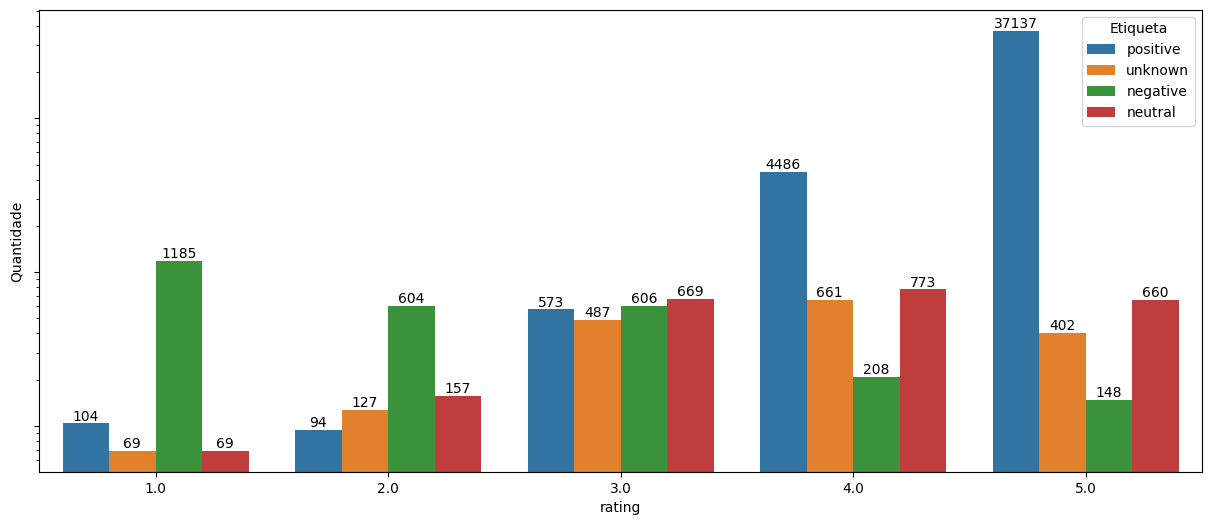
\includegraphics[width=1\textwidth]{figs/vicuna/sentimento_nota.png}
	\caption{\textit{Vicuna} - Sentimento das avaliações por nota}
	\label{img:vicuna_sentimento_nota}
\end{figure}

Os resultados indicam que o \textit{Vicuna} concordam com o modelo \textit{GPT} em quase 89\% das avaliações, conforme Figura~\ref{img:vicuna_vs_gpt}, mostrando uma alta taxa de concordância geral entre os modelos na identificação de sentimentos. Essa elevada consistência sugere que ambos os modelos são eficazes na tarefa, especialmente em relação às avaliações positivas.

\begin{figure}
	\centering
	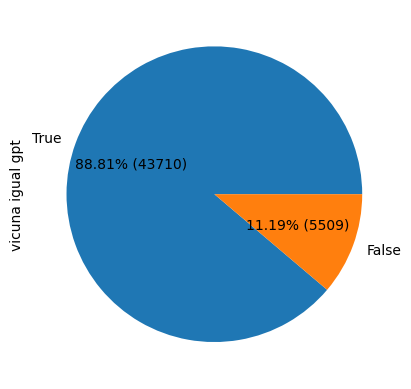
\includegraphics{figs/vicuna/vs_gpt.png}
	\caption{\textit{Vicuna} com sentimento igual ao GPT}
	\label{img:vicuna_vs_gpt}
\end{figure}

No entanto, a Figura~\ref{img:heat_vicuna_vs_gpt} revela áreas de discordância, principalmente nas avaliações negativas, neutras e as que ambos não conseguiram classificar. Embora ambos os modelos concordem fortemente nas classificações positivas, com 40.425 avaliações coincidentes, há uma divergência considerável nas outras categorias, com destaque para as avaliações onde o \textit{Vicuna} classificou como neutro e o \textit{GPT} classificou como negativo. Isso sugere que os modelos podem ter abordagens diferentes para sentimentos mais ambíguos ou menos claros.

\begin{figure}
	\centering
	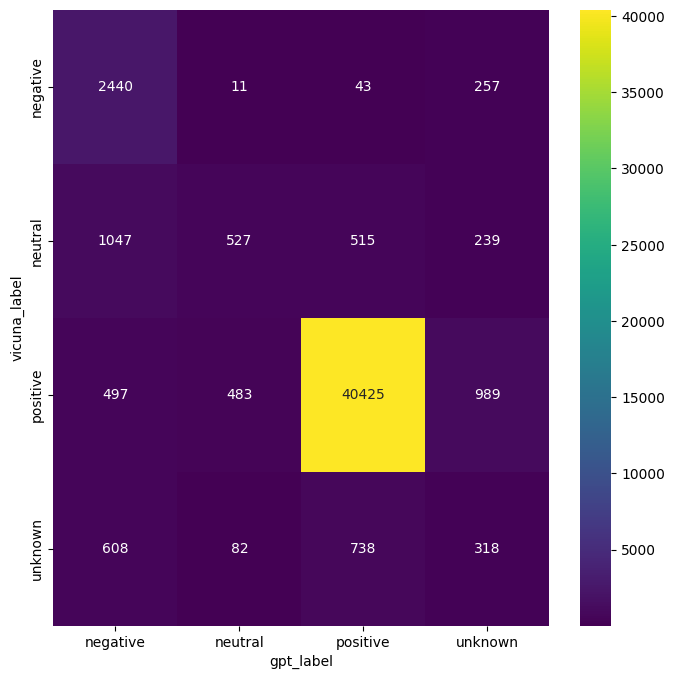
\includegraphics[width=.8\textwidth]{figs/vicuna/heat_vs_gpt.png}
	\caption{Distribuição de sentimento \textit{Vicuna} comparado com GPT}
	\label{img:heat_vicuna_vs_gpt}
\end{figure}


\subsection{GPT 3.5}
\label{sec:resultados:subsec:gpt}

%TODO revisar imagens

O modelo \textit{GPT} 3.5 demorou pouco mais do que 4 horas e teve custo de pouco menos de 11 dólares para realizar a tarefa de atribuição de etiqueta para cada uma das avaliações, além de ser um modelo pago e privado, o que é pode ser um ponto negativo dependendo do projeto que se está executando, ele demorou um tempo consideravelmente maior se comparado com os modelos \textit{BERTs} e para a tarefa proposta no trabalho ambos realizaram uma simular em termos de volume de etiquetas atribuídas para as avaliações, ambos reconheceram como sendo positivas a grande parte, mais de 84\% das avaliações, e o segundo maior grupo como sendo as avaliações negativas.

Outra grande desvantagem do \textit{GPT} é que se faz necessário uso de rede de internet nesse caso, por conta do modelo ser executado na nuvem da OpenAI, que acaba por gerar exposição desnecessária dos dados se comparado com modelos abertos que podem ser executados sem a necessidade de utilização da internet.

Utilizando o modelo \textit{GPT} 3.5 para realizar a tarefa de análise de sentimentos do conteúdo textual das avaliações obtemos a distribuição conforme Figura~\ref{img:gpt_pizza_distribuicao}, onde 84.77\% das avaliações, ou seja, 41721 avaliações foram classificadas como tendo um sentimento positivo, isso representa um número próximo das avaliações que receberam como nota 4 ou 5, 6128 e 38347 avaliações respectivamente, porém fica fácil notar na Figura~\ref{img:gpt_sentimento_nota} que mesmo a grande maioria das avaliações com essa nota atribuída ainda existem avaliações com sentimentos diferentes e até mesmo avaliações em quais a etiqueta atribuída não foi identificável, sendo assim marcadas como com a etiqueta \textit{UNKNOWN}, que foram classificadas dessa forma por conta do modelo não conseguir realizar a tarefa que lhe foi atribuída e produzir resposta maior ou mais detalhada sobre a etiqueta, e como o interesse é em classificações simples e diretas a etiqueta atribuída não foi identificável, mas diferente do que aconteceu com o \textit{Vicuna}, o \textit{GPT} teve mais dificuldade e não foi possível identificar o sentimento atribuído para mais avaliações do que o seu concorrente(1803 vs 1746), sendo o grupo de avaliações com problema na classificação um grupo com maior quantidade de avaliações, 1803(3.66\%) se comparado com o grupo de sentimento neutro, 1103(2.24\%).

\begin{figure}
	\centering
	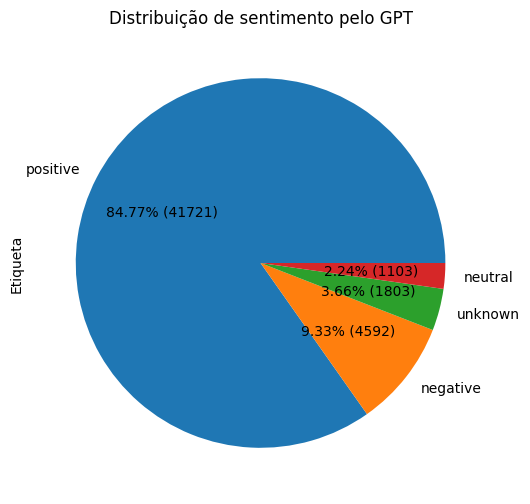
\includegraphics{figs/gpt/distribuicao_pizza.png}
	\caption{GPT - Distribuição do sentimento das avaliações}
	\label{img:gpt_pizza_distribuicao}
\end{figure}
\begin{figure}
	\centering
	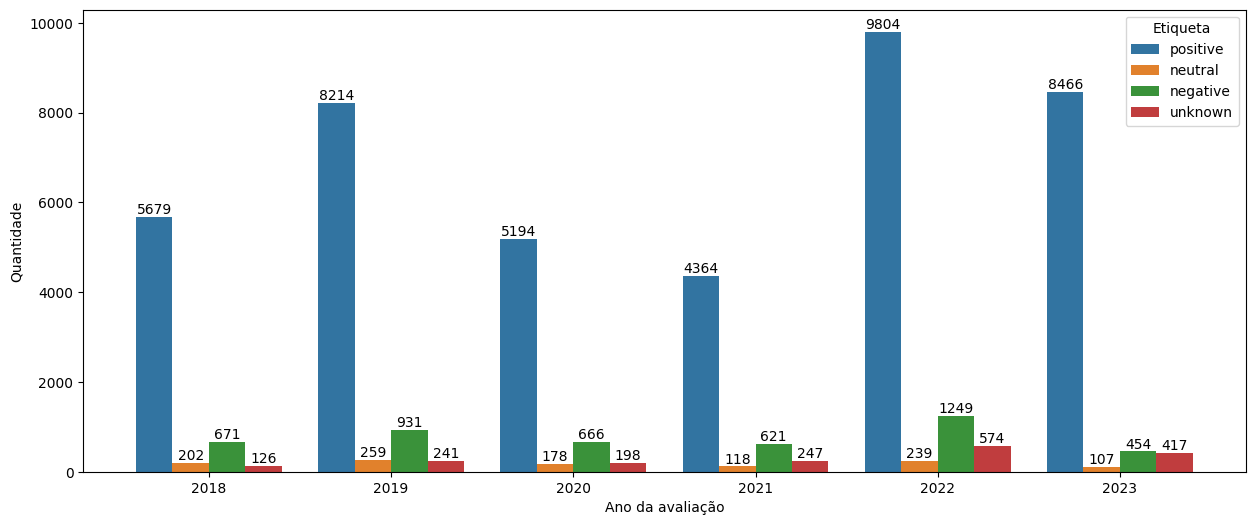
\includegraphics[width=1\textwidth]{figs/gpt/sentimento_ano.png}
	\caption{GPT - Sentimento das avaliações por ano}
	\label{img:gpt_sentimento_ano}
\end{figure}
\begin{figure}
	\centering
	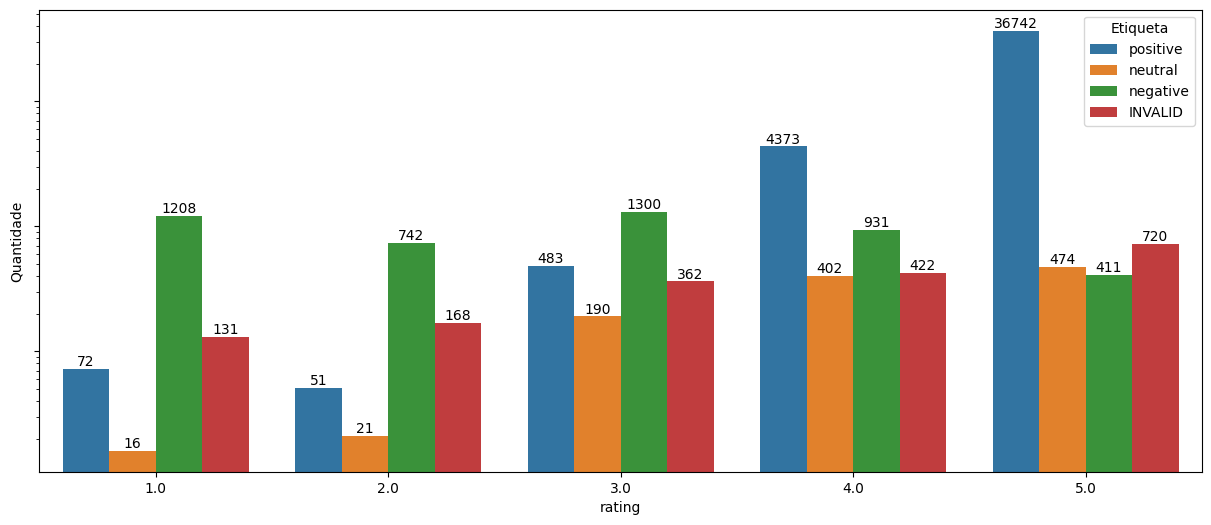
\includegraphics[width=1\textwidth]{figs/gpt/sentimento_nota.png}
	\caption{GPT - Sentimento das avaliações por nota}
	\label{img:gpt_sentimento_nota}
\end{figure}


\subsection{OpenChat}
\label{sec:resultados:subsec:openchat}

%TODO revisar imagens

O modelo OpenChat demorou aproximadamente 9 horas para realizar a tarefa de atribuição de etiqueta para cada uma das avaliações, por ser um modelo menor é esperado que seu desempenho seja inferior se comparado com os anteriores, seu tamanho menor pode ser também um ponto positivo por conta de serem necessários uma menor quantidade de memória de vídeo para carregar o modelo e conseguir realizar a execução do mesmo, ele demorou um tempo consideravelmente maior se comparado com todas as outras abordagens do projeto e para a tarefa proposta no trabalho a atribuição ainda foi simular, reconheceu como sendo positivas a grande parte, aproximadamente 83\% das avaliações, porém o grande destaque está no segundo maior grupo, que é o das avaliações que não foram possíveis classificar, com pouco mais de 11\%.

É perceptível que o modelo do OpenChat não conseguiu executar um bom trabalho com o texto utilizado para iniciar a tarefa se comparado com os outros LLMs, porém ele matem o comportamento esperado de ter um número de avaliações com sentimento positivo bastante destoante dos outros grupos.


\begin{figure}
	\centering
	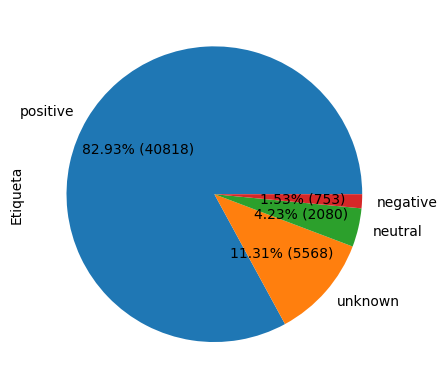
\includegraphics{figs/openchat/distribuicao_pizza.png}
	\caption{OpenChat - Distribuição do sentimento das avaliações}
	\label{img:openchat_pizza_distribuicao}
\end{figure}

\begin{figure}
	\centering
	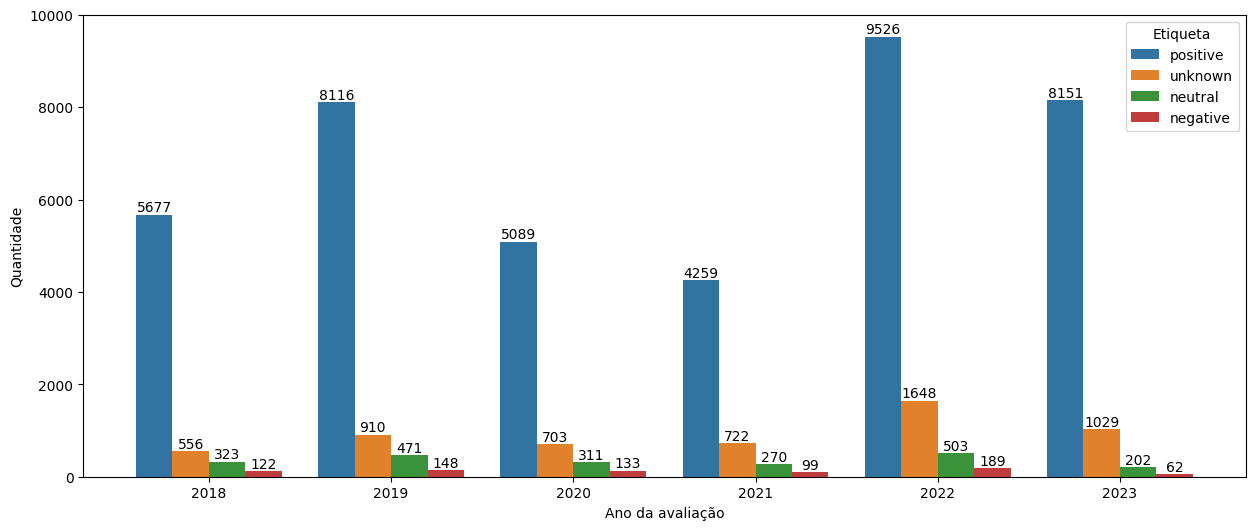
\includegraphics[width=1\textwidth]{figs/openchat/sentimento_ano.png}
	\caption{OpenChat - Sentimento das avaliações por ano}
	\label{img:openchat_sentimento_ano}
\end{figure}

\begin{figure}
	\centering
	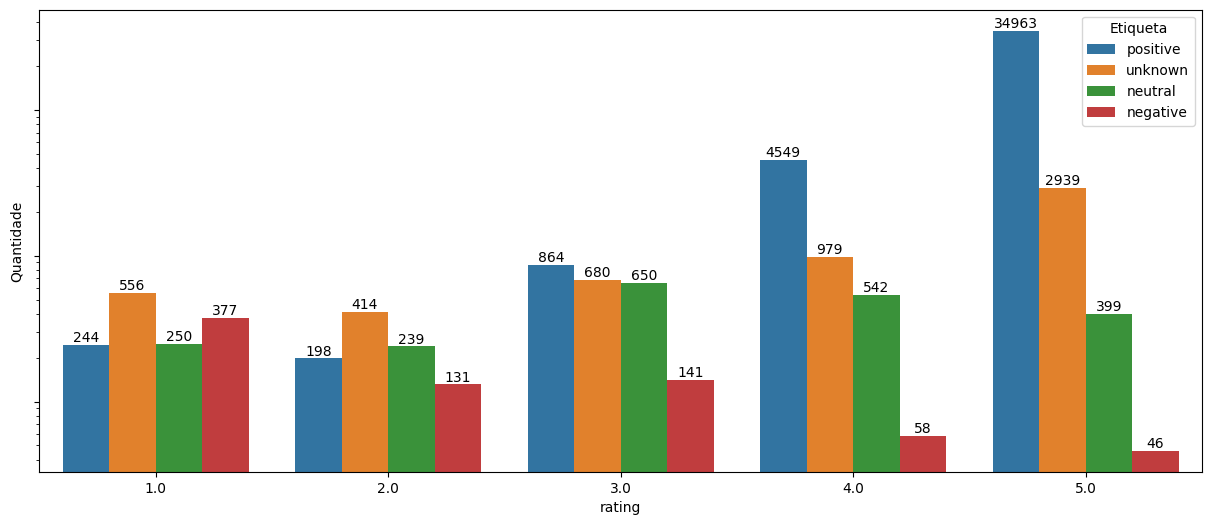
\includegraphics[width=1\textwidth]{figs/openchat/sentimento_nota.png}
	\caption{OpenChat - Sentimento das avaliações por nota}
	\label{img:openchat_sentimento_nota}
\end{figure}

HEAT MAPS.

\begin{figure}
	\centering
	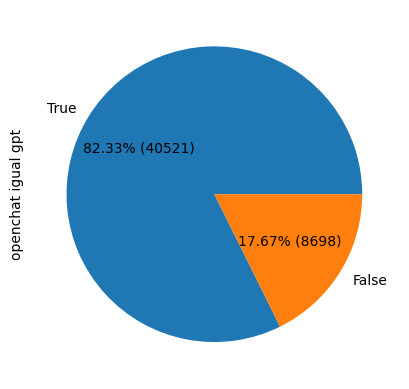
\includegraphics{figs/openchat/vs_gpt.png}
	\caption{OpenChat com sentimento igual ao GPT}
	\label{img:openchat_vs_gpt}
\end{figure}

\begin{figure}
	\centering
	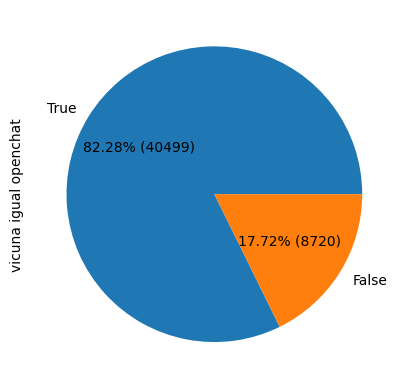
\includegraphics{figs/openchat/vs_vicuna.png}
	\caption{OpenChat com sentimento igual ao \textit{Vicuna}}
	\label{img:openchat_vs_vicuna}
\end{figure}

\begin{figure}
	\centering
	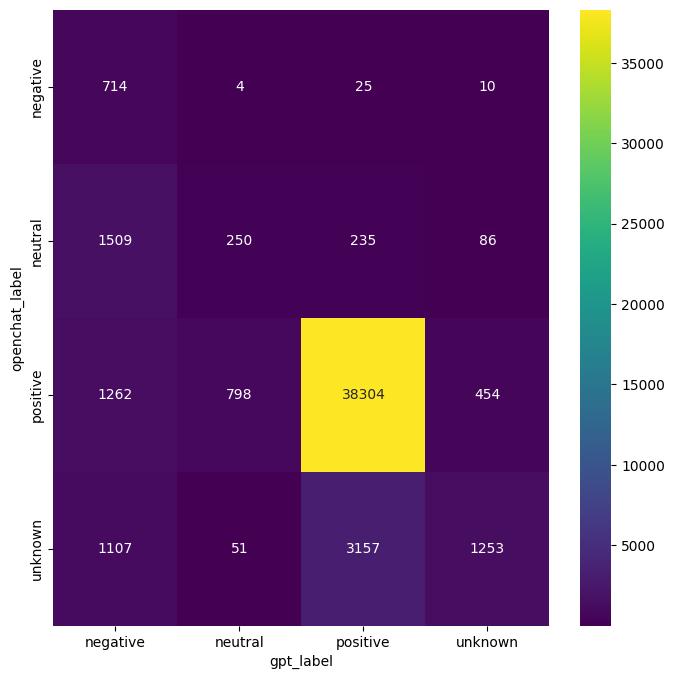
\includegraphics[width=.8\textwidth]{figs/openchat/heat_vs_gpt.png}
	\caption{Distribuição de sentimento OpenChat comparado com GPT}
	\label{img:heat_openchat_vs_gpt}
\end{figure}

\begin{figure}
	\centering
	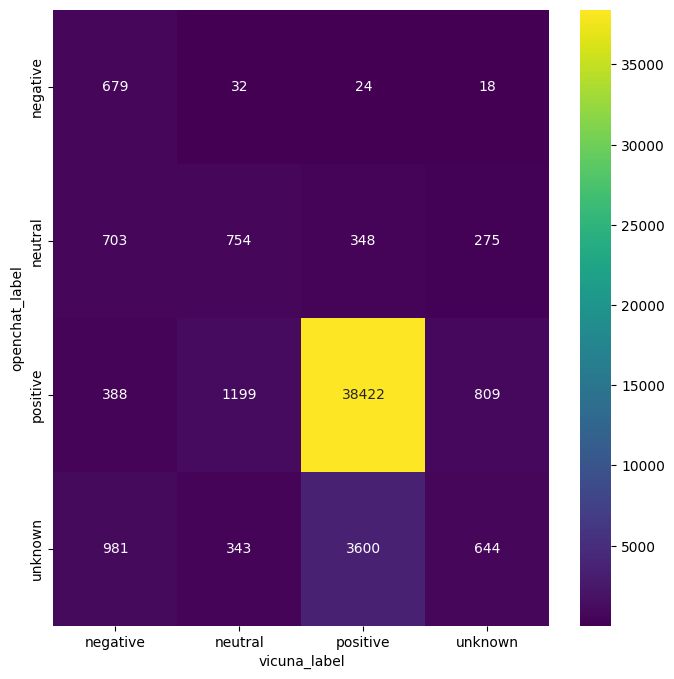
\includegraphics[width=.8\textwidth]{figs/openchat/heat_vs_vicuna.png}
	\caption{Distribuição de sentimento OpenChat comparado com \textit{Vicuna}}
	\label{img:heat_openchat_vs_vicuna}
\end{figure}

\begin{figure}
	\centering
	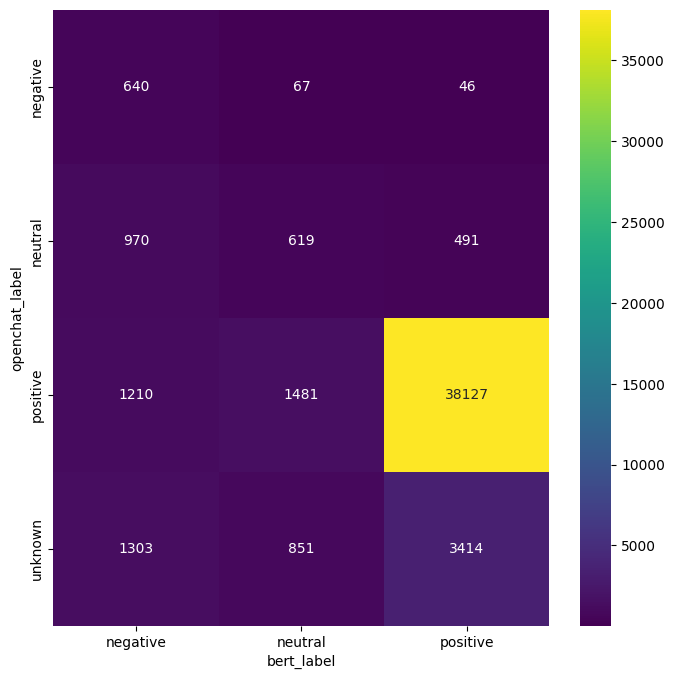
\includegraphics[width=.8\textwidth]{figs/openchat/heat_vs_bert.png}
	\caption{Distribuição de sentimento OpenChat comparado com \textit{BERTs}}
	\label{img:heat_openchat_vs_bert}
\end{figure}


Analisando algumas das classificações que o OpenChat realizou, especificamente contendo o texto \textit{Sem palavras}, temos o total de 7 avaliações com o mesmo texto, todas com uma nota de 5 estrelas atribuída pelo usuário, que não foi levada em consideração no momento de análise, o que é interessante notar é que o GPT classifica todas como sendo de sentimento neutro, já o \textit{Vicuna} classifica como sendo sentimento positivo, porém o OpenChat classifica 5 como tendo o sentimento positivo e as outras duas como sendo de sentimento neutro, o que pode indicar que o ambiente de testes não estava devidamente configurado para que a reprodutividade com esse modelo fosse algo consistente ou que o modelo tem certa inconsistência.

\chapter{Conclusões}
\label{cap:conclusao}
\section{Contribuições}
% TODO

Esse projeto contribui mostrando que para tarefas simples de classificação de sentimento a nível de documento não se faz necessário utilização de grandes modelos complexos, ainda obtemos um bom resultado considerando o uso de recursos e o tempo gasto para realizar a tarefa utilizando apenas os modelos BERT.

\section{Limitações}
% TODO

Uma das limitações desse trabalho é em relação aos recursos disponíveis para execução dos modelos abertos, por conta do ambiente de execução utilizado possuir apenas 12 GB de VRAM não foi possível realizar testes com modelos maiores, e um outro grande impacto é em relação ao texto utilizado como inicio da conversação com cada modelo, onde alguns modelos podem ser mais sensíveis ao texto utilizado para inciar a tarefa de classificação do texto da avaliação.


\section{Trabalhos Futuros}
% TODO

Para trabalhos futuros podemos explorar a analise de impacto do texto inicial utilizado para que o modelo realize a tarefa, e entender a sensibilidade dos modelos para com as alterações no conteúdo utilizado como estimulo para inicio do processamento, bem como o impacto da utilização de modelos iguais porém com tamanho de parâmetros diferentes.

Algo interessante para ser explorado é a utilização de um corpos com uma variação maior de nota de classificação para tentar identificar uma variação de sentimento maior com relação ao tempo, ou até uma possível exploração com maior detalhe utilizando o poder de processamento dos grandes modelos de linguagem, fazendo com que a tarefa não seja uma simples atribuição de etiqueta de sentimento, mas também identificação do sentimento das entidades presentes nos documentos, isto é, o sentimento especifico para uma dada característica do hotel, ou até inverter e no lugar de olhar o conjunto de avaliaçõies de um dado estabelecimento passar a olhar para o conjunto de avaliações de uma lista de local guides e entender a relação de sentimento de suas avaliações e a nota atribuida.



% ----------------------------------------------------------
% ELEMENTOS PÓS-TEXTUAIS (Referências, Glossário, Apêndices)
% ----------------------------------------------------------
\postextual
% Referências bibliográficas
\bibliography{bibliografia}


% Glossário (Consulte o manual)
%\glossary

% Apêndices
% % ----------------------------------------------------------
% Apêndices
% ----------------------------------------------------------

% ---
% Inicia os apêndices
% ---
\begin{apendicesenv}

% Imprime uma página indicando o início dos apêndices
\partapendices

% ----------------------------------------------------------
\chapter{Primeiro Apêndice}
% ----------------------------------------------------------

\begin{figure}
  \centering
  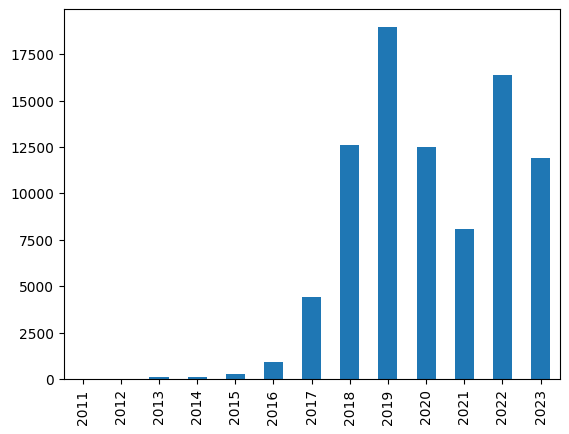
\includegraphics[width=0.75\textwidth]{figs/exploratoria/distribuicao_ano_avaliacao.png}
  \caption{Distribuição do número de avaliação por ano}
  \label{img:dist_ano_avaliacao}
\end{figure}

\end{apendicesenv}


% Anexos
%% ----------------------------------------------------------
% Apêndices
% ----------------------------------------------------------

% ---
% Inicia os anexos
% ---
\begin{anexosenv}

% Imprime uma página indicando o início dos anexos
\partanexos

% ---
\chapter{Nome do Primeiro Anexo}
% ---
\lipsum[30] % Texto qualquer. REMOVER!!

% ---
\chapter{Nome de Outro Anexo}
% ---

\lipsum[32] % Texto qualquer. REMOVER!!

\end{anexosenv}

% Índice remissivo (Consultar manual)
%\phantompart
%\printindex

\end{document}
